\begin{tikzpicture}[scale=.2, anchor=south west]
\node[draw=black, rectangle split, rectangle split parts=2] (sn0x93c9b40W-5) at (-5.5, -12) {
\begin{tikzpicture}[scale=.2]
\node[circle, scale=0.75, fill] (tid0) at (4.5,0){};
\node[circle, scale=0.75, fill] (tid1) at (2.25,1.5){};
\node[circle, scale=0.75, fill, red] (tid4) at (0.75,3){};
\node[circle, scale=0.75, fill, red] (tid5) at (2.25,3){};
\node[circle, scale=0.75, fill] (tid6) at (3.75,3){};
\draw[](tid1) -- (tid4);
\draw[](tid1) -- (tid5);
\draw[](tid1) -- (tid6);
\node[circle, scale=0.75, fill] (tid2) at (6,1.5){};
\node[circle, scale=0.75, fill] (tid7) at (5.25,3){};
\node[circle, scale=0.75, fill] (tid8) at (6.75,3){};
\draw[](tid2) -- (tid7);
\draw[](tid2) -- (tid8);
\node[circle, scale=0.75, fill] (tid3) at (8.25,1.5){};
\node[circle, scale=0.75, fill] (tid9) at (8.25,3){};
\draw[](tid3) -- (tid9);
\draw[](tid0) -- (tid1);
\draw[](tid0) -- (tid2);
\draw[](tid0) -- (tid3);

\end{tikzpicture}
\nodepart{two}
\footnotesize{6.125}
};
\node[draw=black, rectangle split, rectangle split parts=2] (sn0x93d17a0W-14) at (-14.25, -24) {
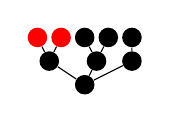
\begin{tikzpicture}[scale=.2]
\node[circle, scale=0.75, fill] (tid0) at (3.75,0){};
\node[circle, scale=0.75, fill] (tid1) at (1.5,1.5){};
\node[circle, scale=0.75, fill, red] (tid4) at (0.75,3){};
\node[circle, scale=0.75, fill, red] (tid5) at (2.25,3){};
\draw[](tid1) -- (tid4);
\draw[](tid1) -- (tid5);
\node[circle, scale=0.75, fill] (tid2) at (4.5,1.5){};
\node[circle, scale=0.75, fill] (tid6) at (3.75,3){};
\node[circle, scale=0.75, fill] (tid7) at (5.25,3){};
\draw[](tid2) -- (tid6);
\draw[](tid2) -- (tid7);
\node[circle, scale=0.75, fill] (tid3) at (6.75,1.5){};
\node[circle, scale=0.75, fill] (tid8) at (6.75,3){};
\draw[](tid3) -- (tid8);
\draw[](tid0) -- (tid1);
\draw[](tid0) -- (tid2);
\draw[](tid0) -- (tid3);

\end{tikzpicture}
\nodepart{two}
\footnotesize{5.625}
};
\node[draw=black, rectangle split, rectangle split parts=2] (sn0x93d1558W-25) at (-25.5, -36) {
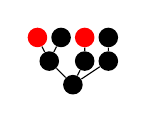
\begin{tikzpicture}[scale=.2]
\node[circle, scale=0.75, fill] (tid0) at (3,0){};
\node[circle, scale=0.75, fill] (tid1) at (1.5,1.5){};
\node[circle, scale=0.75, fill, red] (tid4) at (0.75,3){};
\node[circle, scale=0.75, fill] (tid5) at (2.25,3){};
\draw[](tid1) -- (tid4);
\draw[](tid1) -- (tid5);
\node[circle, scale=0.75, fill] (tid2) at (3.75,1.5){};
\node[circle, scale=0.75, fill, red] (tid6) at (3.75,3){};
\draw[](tid2) -- (tid6);
\node[circle, scale=0.75, fill] (tid3) at (5.25,1.5){};
\node[circle, scale=0.75, fill] (tid7) at (5.25,3){};
\draw[](tid3) -- (tid7);
\draw[](tid0) -- (tid1);
\draw[](tid0) -- (tid2);
\draw[](tid0) -- (tid3);

\end{tikzpicture}
\nodepart{two}
\footnotesize{5.125}
};
\node[draw=black, rectangle split, rectangle split parts=2] (sn0x93d0fa8W-17) at (-17.75, -48) {
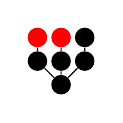
\begin{tikzpicture}[scale=.2]
\node[circle, scale=0.75, fill] (tid0) at (2.25,0){};
\node[circle, scale=0.75, fill] (tid1) at (0.75,1.5){};
\node[circle, scale=0.75, fill, red] (tid4) at (0.75,3){};
\draw[](tid1) -- (tid4);
\node[circle, scale=0.75, fill] (tid2) at (2.25,1.5){};
\node[circle, scale=0.75, fill, red] (tid5) at (2.25,3){};
\draw[](tid2) -- (tid5);
\node[circle, scale=0.75, fill] (tid3) at (3.75,1.5){};
\node[circle, scale=0.75, fill] (tid6) at (3.75,3){};
\draw[](tid3) -- (tid6);
\draw[](tid0) -- (tid1);
\draw[](tid0) -- (tid2);
\draw[](tid0) -- (tid3);

\end{tikzpicture}
\nodepart{two}
\footnotesize{4.625}
};
\node[draw=black, rectangle split, rectangle split parts=2] (sn0x93cb870W-7) at (-7.25, -60) {
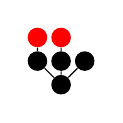
\begin{tikzpicture}[scale=.2]
\node[circle, scale=0.75, fill] (tid0) at (2.25,0){};
\node[circle, scale=0.75, fill] (tid1) at (0.75,1.5){};
\node[circle, scale=0.75, fill, red] (tid4) at (0.75,3){};
\draw[](tid1) -- (tid4);
\node[circle, scale=0.75, fill] (tid2) at (2.25,1.5){};
\node[circle, scale=0.75, fill, red] (tid5) at (2.25,3){};
\draw[](tid2) -- (tid5);
\node[circle, scale=0.75, fill] (tid3) at (3.75,1.5){};
\draw[](tid0) -- (tid1);
\draw[](tid0) -- (tid2);
\draw[](tid0) -- (tid3);

\end{tikzpicture}
\nodepart{two}
\footnotesize{4.125}
};
\node[draw=black, rectangle split, rectangle split parts=2] (sn0x93ca478W-3) at (-3.25, -72) {
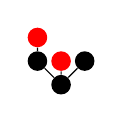
\begin{tikzpicture}[scale=.2]
\node[circle, scale=0.75, fill] (tid0) at (2.25,0){};
\node[circle, scale=0.75, fill] (tid1) at (0.75,1.5){};
\node[circle, scale=0.75, fill, red] (tid4) at (0.75,3){};
\draw[](tid1) -- (tid4);
\node[circle, scale=0.75, fill, red] (tid2) at (2.25,1.5){};
\node[circle, scale=0.75, fill] (tid3) at (3.75,1.5){};
\draw[](tid0) -- (tid1);
\draw[](tid0) -- (tid2);
\draw[](tid0) -- (tid3);

\end{tikzpicture}
\nodepart{two}
\footnotesize{3.625}
};
\node[draw=black, rectangle split, rectangle split parts=2] (sn0x93ca4e0W-5) at (-5.75, -84) {
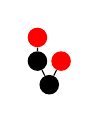
\begin{tikzpicture}[scale=.2]
\node[circle, scale=0.75, fill] (tid0) at (1.5,0){};
\node[circle, scale=0.75, fill] (tid1) at (0.75,1.5){};
\node[circle, scale=0.75, fill, red] (tid3) at (0.75,3){};
\draw[](tid1) -- (tid3);
\node[circle, scale=0.75, fill, red] (tid2) at (2.25,1.5){};
\draw[](tid0) -- (tid1);
\draw[](tid0) -- (tid2);

\end{tikzpicture}
\nodepart{two}
\footnotesize{3.25}
};
\node[draw=black, rectangle split, rectangle split parts=2] (sn0x93d1938W-4) at (-4.25, -96) {
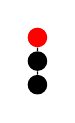
\begin{tikzpicture}[scale=.2]
\node[circle, scale=0.75, fill] (tid0) at (0.75,0){};
\node[circle, scale=0.75, fill] (tid1) at (0.75,1.5){};
\node[circle, scale=0.75, fill, red] (tid2) at (0.75,3){};
\draw[](tid1) -- (tid2);
\draw[](tid0) -- (tid1);

\end{tikzpicture}
\nodepart{two}
\footnotesize{3}
};
\node[draw=black, rectangle split, rectangle split parts=2] (sn0x93d1c08W-1) at (-1.75, -108) {

\begin{tikzpicture}[scale=.2]
\node[circle, scale=0.75, fill] (tid0) at (0.75,0){};
\node[circle, scale=0.75, fill, red] (tid1) at (0.75,1.5){};
\draw[](tid0) -- (tid1);

\end{tikzpicture}
\nodepart{two}
\footnotesize{2}
};
\draw (sn0x93d1938W-4.south) -- (sn0x93d1c08W-1.north);
\node[draw=black, rectangle split, rectangle split parts=2] (sn0x93d1a28W0) at (-0.75, -96) {

\begin{tikzpicture}[scale=.2]
\node[circle, scale=0.75, fill] (tid0) at (1.5,0){};
\node[circle, scale=0.75, fill, red] (tid1) at (0.75,1.5){};
\node[circle, scale=0.75, fill, red] (tid2) at (2.25,1.5){};
\draw[](tid0) -- (tid1);
\draw[](tid0) -- (tid2);

\end{tikzpicture}
\nodepart{two}
\footnotesize{2.5}
};
\draw (sn0x93d1a28W0.south) -- (sn0x93d1c08W-1.north);
\draw (sn0x93ca4e0W-5.south) -- (sn0x93d1938W-4.north);
\draw (sn0x93ca4e0W-5.south) -- (sn0x93d1a28W0.north);
\node[draw=black, rectangle split, rectangle split parts=2] (sn0x93cab38W0) at (-0.75, -84) {
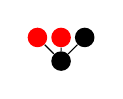
\begin{tikzpicture}[scale=.2]
\node[circle, scale=0.75, fill] (tid0) at (2.25,0){};
\node[circle, scale=0.75, fill, red] (tid1) at (0.75,1.5){};
\node[circle, scale=0.75, fill, red] (tid2) at (2.25,1.5){};
\node[circle, scale=0.75, fill] (tid3) at (3.75,1.5){};
\draw[](tid0) -- (tid1);
\draw[](tid0) -- (tid2);
\draw[](tid0) -- (tid3);

\end{tikzpicture}
\nodepart{two}
\footnotesize{3}
};
\draw (sn0x93cab38W0.south) -- (sn0x93d1a28W0.north);
\draw (sn0x93ca478W-3.south) -- (sn0x93ca4e0W-5.north);
\draw (sn0x93ca478W-3.south) -- (sn0x93cab38W0.north);
\draw (sn0x93cb870W-7.south) -- (sn0x93ca478W-3.north);
\draw (sn0x93d0fa8W-17.south) -- (sn0x93cb870W-7.north);
\node[draw=black, rectangle split, rectangle split parts=2] (sn0x93cb048W-11) at (-11.25, -48) {
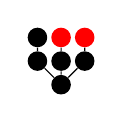
\begin{tikzpicture}[scale=.2]
\node[circle, scale=0.75, fill] (tid0) at (2.25,0){};
\node[circle, scale=0.75, fill] (tid1) at (0.75,1.5){};
\node[circle, scale=0.75, fill] (tid4) at (0.75,3){};
\draw[](tid1) -- (tid4);
\node[circle, scale=0.75, fill] (tid2) at (2.25,1.5){};
\node[circle, scale=0.75, fill, red] (tid5) at (2.25,3){};
\draw[](tid2) -- (tid5);
\node[circle, scale=0.75, fill] (tid3) at (3.75,1.5){};
\node[circle, scale=0.75, fill, red] (tid6) at (3.75,3){};
\draw[](tid3) -- (tid6);
\draw[](tid0) -- (tid1);
\draw[](tid0) -- (tid2);
\draw[](tid0) -- (tid3);

\end{tikzpicture}
\nodepart{two}
\footnotesize{4.625}
};
\draw (sn0x93cb048W-11.south) -- (sn0x93cb870W-7.north);
\node[draw=black, rectangle split, rectangle split parts=2] (sn0x93ca858W-4) at (-4.75, -48) {
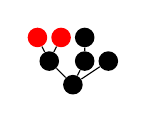
\begin{tikzpicture}[scale=.2]
\node[circle, scale=0.75, fill] (tid0) at (3,0){};
\node[circle, scale=0.75, fill] (tid1) at (1.5,1.5){};
\node[circle, scale=0.75, fill, red] (tid4) at (0.75,3){};
\node[circle, scale=0.75, fill, red] (tid5) at (2.25,3){};
\draw[](tid1) -- (tid4);
\draw[](tid1) -- (tid5);
\node[circle, scale=0.75, fill] (tid2) at (3.75,1.5){};
\node[circle, scale=0.75, fill] (tid6) at (3.75,3){};
\draw[](tid2) -- (tid6);
\node[circle, scale=0.75, fill] (tid3) at (5.25,1.5){};
\draw[](tid0) -- (tid1);
\draw[](tid0) -- (tid2);
\draw[](tid0) -- (tid3);

\end{tikzpicture}
\nodepart{two}
\footnotesize{4.625}
};
\draw (sn0x93ca858W-4.south) -- (sn0x93cb870W-7.north);
\node[draw=black, rectangle split, rectangle split parts=2] (sn0x93cb808W3) at (3.25, -48) {
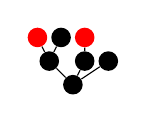
\begin{tikzpicture}[scale=.2]
\node[circle, scale=0.75, fill] (tid0) at (3,0){};
\node[circle, scale=0.75, fill] (tid1) at (1.5,1.5){};
\node[circle, scale=0.75, fill, red] (tid4) at (0.75,3){};
\node[circle, scale=0.75, fill] (tid5) at (2.25,3){};
\draw[](tid1) -- (tid4);
\draw[](tid1) -- (tid5);
\node[circle, scale=0.75, fill] (tid2) at (3.75,1.5){};
\node[circle, scale=0.75, fill, red] (tid6) at (3.75,3){};
\draw[](tid2) -- (tid6);
\node[circle, scale=0.75, fill] (tid3) at (5.25,1.5){};
\draw[](tid0) -- (tid1);
\draw[](tid0) -- (tid2);
\draw[](tid0) -- (tid3);

\end{tikzpicture}
\nodepart{two}
\footnotesize{4.625}
};
\node[draw=black, rectangle split, rectangle split parts=2] (sn0x93d2048W0) at (-0.75, -60) {
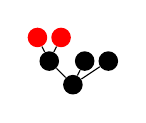
\begin{tikzpicture}[scale=.2]
\node[circle, scale=0.75, fill] (tid0) at (3,0){};
\node[circle, scale=0.75, fill] (tid1) at (1.5,1.5){};
\node[circle, scale=0.75, fill, red] (tid4) at (0.75,3){};
\node[circle, scale=0.75, fill, red] (tid5) at (2.25,3){};
\draw[](tid1) -- (tid4);
\draw[](tid1) -- (tid5);
\node[circle, scale=0.75, fill] (tid2) at (3.75,1.5){};
\node[circle, scale=0.75, fill] (tid3) at (5.25,1.5){};
\draw[](tid0) -- (tid1);
\draw[](tid0) -- (tid2);
\draw[](tid0) -- (tid3);

\end{tikzpicture}
\nodepart{two}
\footnotesize{4.125}
};
\draw (sn0x93d2048W0.south) -- (sn0x93ca478W-3.north);
\draw (sn0x93cb808W3.south) -- (sn0x93cb870W-7.north);
\draw (sn0x93cb808W3.south) -- (sn0x93d2048W0.north);
\draw (sn0x93d1558W-25.south) -- (sn0x93d0fa8W-17.north);
\draw (sn0x93d1558W-25.south) -- (sn0x93cb048W-11.north);
\draw (sn0x93d1558W-25.south) -- (sn0x93ca858W-4.north);
\draw (sn0x93d1558W-25.south) -- (sn0x93cb808W3.north);
\node[draw=black, rectangle split, rectangle split parts=2] (sn0x93c8a38W-17) at (-17.5, -36) {
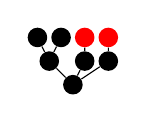
\begin{tikzpicture}[scale=.2]
\node[circle, scale=0.75, fill] (tid0) at (3,0){};
\node[circle, scale=0.75, fill] (tid1) at (1.5,1.5){};
\node[circle, scale=0.75, fill] (tid4) at (0.75,3){};
\node[circle, scale=0.75, fill] (tid5) at (2.25,3){};
\draw[](tid1) -- (tid4);
\draw[](tid1) -- (tid5);
\node[circle, scale=0.75, fill] (tid2) at (3.75,1.5){};
\node[circle, scale=0.75, fill, red] (tid6) at (3.75,3){};
\draw[](tid2) -- (tid6);
\node[circle, scale=0.75, fill] (tid3) at (5.25,1.5){};
\node[circle, scale=0.75, fill, red] (tid7) at (5.25,3){};
\draw[](tid3) -- (tid7);
\draw[](tid0) -- (tid1);
\draw[](tid0) -- (tid2);
\draw[](tid0) -- (tid3);

\end{tikzpicture}
\nodepart{two}
\footnotesize{5.125}
};
\draw (sn0x93c8a38W-17.south) -- (sn0x93cb808W3.north);
\draw (sn0x93d17a0W-14.south) -- (sn0x93d1558W-25.north);
\draw (sn0x93d17a0W-14.south) -- (sn0x93c8a38W-17.north);
\node[draw=black, rectangle split, rectangle split parts=2] (sn0x93c8458W-4) at (-4.75, -24) {
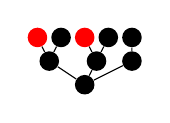
\begin{tikzpicture}[scale=.2]
\node[circle, scale=0.75, fill] (tid0) at (3.75,0){};
\node[circle, scale=0.75, fill] (tid1) at (1.5,1.5){};
\node[circle, scale=0.75, fill, red] (tid4) at (0.75,3){};
\node[circle, scale=0.75, fill] (tid5) at (2.25,3){};
\draw[](tid1) -- (tid4);
\draw[](tid1) -- (tid5);
\node[circle, scale=0.75, fill] (tid2) at (4.5,1.5){};
\node[circle, scale=0.75, fill, red] (tid6) at (3.75,3){};
\node[circle, scale=0.75, fill] (tid7) at (5.25,3){};
\draw[](tid2) -- (tid6);
\draw[](tid2) -- (tid7);
\node[circle, scale=0.75, fill] (tid3) at (6.75,1.5){};
\node[circle, scale=0.75, fill] (tid8) at (6.75,3){};
\draw[](tid3) -- (tid8);
\draw[](tid0) -- (tid1);
\draw[](tid0) -- (tid2);
\draw[](tid0) -- (tid3);

\end{tikzpicture}
\nodepart{two}
\footnotesize{5.625}
};
\node[draw=black, rectangle split, rectangle split parts=2] (sn0x93d2660W-9) at (-9.5, -36) {
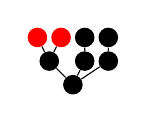
\begin{tikzpicture}[scale=.2]
\node[circle, scale=0.75, fill] (tid0) at (3,0){};
\node[circle, scale=0.75, fill] (tid1) at (1.5,1.5){};
\node[circle, scale=0.75, fill, red] (tid4) at (0.75,3){};
\node[circle, scale=0.75, fill, red] (tid5) at (2.25,3){};
\draw[](tid1) -- (tid4);
\draw[](tid1) -- (tid5);
\node[circle, scale=0.75, fill] (tid2) at (3.75,1.5){};
\node[circle, scale=0.75, fill] (tid6) at (3.75,3){};
\draw[](tid2) -- (tid6);
\node[circle, scale=0.75, fill] (tid3) at (5.25,1.5){};
\node[circle, scale=0.75, fill] (tid7) at (5.25,3){};
\draw[](tid3) -- (tid7);
\draw[](tid0) -- (tid1);
\draw[](tid0) -- (tid2);
\draw[](tid0) -- (tid3);

\end{tikzpicture}
\nodepart{two}
\footnotesize{5.125}
};
\node[draw=black, rectangle split, rectangle split parts=2] (sn0x93d2c08W11) at (11.25, -48) {
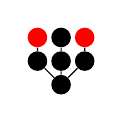
\begin{tikzpicture}[scale=.2]
\node[circle, scale=0.75, fill] (tid0) at (2.25,0){};
\node[circle, scale=0.75, fill] (tid1) at (0.75,1.5){};
\node[circle, scale=0.75, fill, red] (tid4) at (0.75,3){};
\draw[](tid1) -- (tid4);
\node[circle, scale=0.75, fill] (tid2) at (2.25,1.5){};
\node[circle, scale=0.75, fill] (tid5) at (2.25,3){};
\draw[](tid2) -- (tid5);
\node[circle, scale=0.75, fill] (tid3) at (3.75,1.5){};
\node[circle, scale=0.75, fill, red] (tid6) at (3.75,3){};
\draw[](tid3) -- (tid6);
\draw[](tid0) -- (tid1);
\draw[](tid0) -- (tid2);
\draw[](tid0) -- (tid3);

\end{tikzpicture}
\nodepart{two}
\footnotesize{4.625}
};
\draw (sn0x93d2c08W11.south) -- (sn0x93cb870W-7.north);
\draw (sn0x93d2660W-9.south) -- (sn0x93d0fa8W-17.north);
\draw (sn0x93d2660W-9.south) -- (sn0x93d2c08W11.north);
\node[draw=black, rectangle split, rectangle split parts=2] (sn0x93d2868W-1) at (-1.5, -36) {
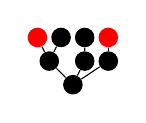
\begin{tikzpicture}[scale=.2]
\node[circle, scale=0.75, fill] (tid0) at (3,0){};
\node[circle, scale=0.75, fill] (tid1) at (1.5,1.5){};
\node[circle, scale=0.75, fill, red] (tid4) at (0.75,3){};
\node[circle, scale=0.75, fill] (tid5) at (2.25,3){};
\draw[](tid1) -- (tid4);
\draw[](tid1) -- (tid5);
\node[circle, scale=0.75, fill] (tid2) at (3.75,1.5){};
\node[circle, scale=0.75, fill] (tid6) at (3.75,3){};
\draw[](tid2) -- (tid6);
\node[circle, scale=0.75, fill] (tid3) at (5.25,1.5){};
\node[circle, scale=0.75, fill, red] (tid7) at (5.25,3){};
\draw[](tid3) -- (tid7);
\draw[](tid0) -- (tid1);
\draw[](tid0) -- (tid2);
\draw[](tid0) -- (tid3);

\end{tikzpicture}
\nodepart{two}
\footnotesize{5.125}
};
\draw (sn0x93d2868W-1.south) -- (sn0x93d2c08W11.north);
\draw (sn0x93d2868W-1.south) -- (sn0x93cb048W-11.north);
\draw (sn0x93d2868W-1.south) -- (sn0x93ca858W-4.north);
\draw (sn0x93d2868W-1.south) -- (sn0x93cb808W3.north);
\draw (sn0x93c8458W-4.south) -- (sn0x93d1558W-25.north);
\draw (sn0x93c8458W-4.south) -- (sn0x93d2660W-9.north);
\draw (sn0x93c8458W-4.south) -- (sn0x93d2868W-1.north);
\node[draw=black, rectangle split, rectangle split parts=2] (sn0x93c90c8W4) at (4.75, -24) {
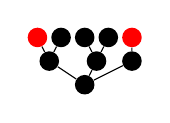
\begin{tikzpicture}[scale=.2]
\node[circle, scale=0.75, fill] (tid0) at (3.75,0){};
\node[circle, scale=0.75, fill] (tid1) at (1.5,1.5){};
\node[circle, scale=0.75, fill, red] (tid4) at (0.75,3){};
\node[circle, scale=0.75, fill] (tid5) at (2.25,3){};
\draw[](tid1) -- (tid4);
\draw[](tid1) -- (tid5);
\node[circle, scale=0.75, fill] (tid2) at (4.5,1.5){};
\node[circle, scale=0.75, fill] (tid6) at (3.75,3){};
\node[circle, scale=0.75, fill] (tid7) at (5.25,3){};
\draw[](tid2) -- (tid6);
\draw[](tid2) -- (tid7);
\node[circle, scale=0.75, fill] (tid3) at (6.75,1.5){};
\node[circle, scale=0.75, fill, red] (tid8) at (6.75,3){};
\draw[](tid3) -- (tid8);
\draw[](tid0) -- (tid1);
\draw[](tid0) -- (tid2);
\draw[](tid0) -- (tid3);

\end{tikzpicture}
\nodepart{two}
\footnotesize{5.625}
};
\node[draw=black, rectangle split, rectangle split parts=2] (sn0x93d2dc8W6) at (6.5, -36) {
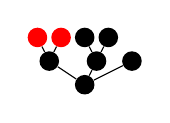
\begin{tikzpicture}[scale=.2]
\node[circle, scale=0.75, fill] (tid0) at (3.75,0){};
\node[circle, scale=0.75, fill] (tid1) at (1.5,1.5){};
\node[circle, scale=0.75, fill, red] (tid4) at (0.75,3){};
\node[circle, scale=0.75, fill, red] (tid5) at (2.25,3){};
\draw[](tid1) -- (tid4);
\draw[](tid1) -- (tid5);
\node[circle, scale=0.75, fill] (tid2) at (4.5,1.5){};
\node[circle, scale=0.75, fill] (tid6) at (3.75,3){};
\node[circle, scale=0.75, fill] (tid7) at (5.25,3){};
\draw[](tid2) -- (tid6);
\draw[](tid2) -- (tid7);
\node[circle, scale=0.75, fill] (tid3) at (6.75,1.5){};
\draw[](tid0) -- (tid1);
\draw[](tid0) -- (tid2);
\draw[](tid0) -- (tid3);

\end{tikzpicture}
\nodepart{two}
\footnotesize{5.125}
};
\draw (sn0x93d2dc8W6.south) -- (sn0x93cb808W3.north);
\node[draw=black, rectangle split, rectangle split parts=2] (sn0x93d2e60W16) at (16, -36) {
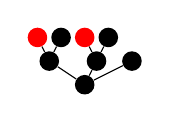
\begin{tikzpicture}[scale=.2]
\node[circle, scale=0.75, fill] (tid0) at (3.75,0){};
\node[circle, scale=0.75, fill] (tid1) at (1.5,1.5){};
\node[circle, scale=0.75, fill, red] (tid4) at (0.75,3){};
\node[circle, scale=0.75, fill] (tid5) at (2.25,3){};
\draw[](tid1) -- (tid4);
\draw[](tid1) -- (tid5);
\node[circle, scale=0.75, fill] (tid2) at (4.5,1.5){};
\node[circle, scale=0.75, fill, red] (tid6) at (3.75,3){};
\node[circle, scale=0.75, fill] (tid7) at (5.25,3){};
\draw[](tid2) -- (tid6);
\draw[](tid2) -- (tid7);
\node[circle, scale=0.75, fill] (tid3) at (6.75,1.5){};
\draw[](tid0) -- (tid1);
\draw[](tid0) -- (tid2);
\draw[](tid0) -- (tid3);

\end{tikzpicture}
\nodepart{two}
\footnotesize{5.125}
};
\draw (sn0x93d2e60W16.south) -- (sn0x93cb808W3.north);
\draw (sn0x93d2e60W16.south) -- (sn0x93ca858W-4.north);
\draw (sn0x93c90c8W4.south) -- (sn0x93c8a38W-17.north);
\draw (sn0x93c90c8W4.south) -- (sn0x93d2868W-1.north);
\draw (sn0x93c90c8W4.south) -- (sn0x93d2dc8W6.north);
\draw (sn0x93c90c8W4.south) -- (sn0x93d2e60W16.north);
\draw (sn0x93c9b40W-5.south) -- (sn0x93d17a0W-14.north);
\draw (sn0x93c9b40W-5.south) -- (sn0x93c8458W-4.north);
\draw (sn0x93c9b40W-5.south) -- (sn0x93c90c8W4.north);
\end{tikzpicture}

%%% Local Variables:
%%% TeX-master: "thesis/thesis.tex"
%%% End: 

\begin{tikzpicture}[scale=.2, anchor=south west]
\node[draw=black, rectangle split, rectangle split parts=2] (sn0x93c9ba0W-5) at (-5.5, -12) {
\begin{tikzpicture}[scale=.2]
\node[circle, scale=0.75, fill] (tid0) at (4.5,0){};
\node[circle, scale=0.75, fill] (tid1) at (2.25,1.5){};
\node[circle, scale=0.75, fill, red] (tid4) at (0.75,3){};
\node[circle, scale=0.75, fill] (tid5) at (2.25,3){};
\node[circle, scale=0.75, fill] (tid6) at (3.75,3){};
\draw[](tid1) -- (tid4);
\draw[](tid1) -- (tid5);
\draw[](tid1) -- (tid6);
\node[circle, scale=0.75, fill] (tid2) at (6,1.5){};
\node[circle, scale=0.75, fill] (tid7) at (5.25,3){};
\node[circle, scale=0.75, fill] (tid8) at (6.75,3){};
\draw[](tid2) -- (tid7);
\draw[](tid2) -- (tid8);
\node[circle, scale=0.75, fill] (tid3) at (8.25,1.5){};
\node[circle, scale=0.75, fill, red] (tid9) at (8.25,3){};
\draw[](tid3) -- (tid9);
\draw[](tid0) -- (tid1);
\draw[](tid0) -- (tid2);
\draw[](tid0) -- (tid3);

\end{tikzpicture}
\nodepart{two}
\footnotesize{6.125}
};
\node[draw=black, rectangle split, rectangle split parts=2] (sn0x93c90c8W-20) at (-20.5, -24) {
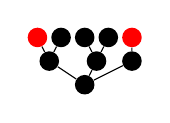
\begin{tikzpicture}[scale=.2]
\node[circle, scale=0.75, fill] (tid0) at (3.75,0){};
\node[circle, scale=0.75, fill] (tid1) at (1.5,1.5){};
\node[circle, scale=0.75, fill, red] (tid4) at (0.75,3){};
\node[circle, scale=0.75, fill] (tid5) at (2.25,3){};
\draw[](tid1) -- (tid4);
\draw[](tid1) -- (tid5);
\node[circle, scale=0.75, fill] (tid2) at (4.5,1.5){};
\node[circle, scale=0.75, fill] (tid6) at (3.75,3){};
\node[circle, scale=0.75, fill] (tid7) at (5.25,3){};
\draw[](tid2) -- (tid6);
\draw[](tid2) -- (tid7);
\node[circle, scale=0.75, fill] (tid3) at (6.75,1.5){};
\node[circle, scale=0.75, fill, red] (tid8) at (6.75,3){};
\draw[](tid3) -- (tid8);
\draw[](tid0) -- (tid1);
\draw[](tid0) -- (tid2);
\draw[](tid0) -- (tid3);

\end{tikzpicture}
\nodepart{two}
\footnotesize{5.625}
};
\node[draw=black, rectangle split, rectangle split parts=2] (sn0x93c8a38W-31) at (-31.75, -36) {
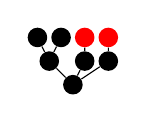
\begin{tikzpicture}[scale=.2]
\node[circle, scale=0.75, fill] (tid0) at (3,0){};
\node[circle, scale=0.75, fill] (tid1) at (1.5,1.5){};
\node[circle, scale=0.75, fill] (tid4) at (0.75,3){};
\node[circle, scale=0.75, fill] (tid5) at (2.25,3){};
\draw[](tid1) -- (tid4);
\draw[](tid1) -- (tid5);
\node[circle, scale=0.75, fill] (tid2) at (3.75,1.5){};
\node[circle, scale=0.75, fill, red] (tid6) at (3.75,3){};
\draw[](tid2) -- (tid6);
\node[circle, scale=0.75, fill] (tid3) at (5.25,1.5){};
\node[circle, scale=0.75, fill, red] (tid7) at (5.25,3){};
\draw[](tid3) -- (tid7);
\draw[](tid0) -- (tid1);
\draw[](tid0) -- (tid2);
\draw[](tid0) -- (tid3);

\end{tikzpicture}
\nodepart{two}
\footnotesize{5.125}
};
\node[draw=black, rectangle split, rectangle split parts=2] (sn0x93cb808W-19) at (-19.25, -48) {
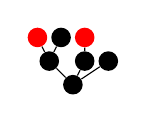
\begin{tikzpicture}[scale=.2]
\node[circle, scale=0.75, fill] (tid0) at (3,0){};
\node[circle, scale=0.75, fill] (tid1) at (1.5,1.5){};
\node[circle, scale=0.75, fill, red] (tid4) at (0.75,3){};
\node[circle, scale=0.75, fill] (tid5) at (2.25,3){};
\draw[](tid1) -- (tid4);
\draw[](tid1) -- (tid5);
\node[circle, scale=0.75, fill] (tid2) at (3.75,1.5){};
\node[circle, scale=0.75, fill, red] (tid6) at (3.75,3){};
\draw[](tid2) -- (tid6);
\node[circle, scale=0.75, fill] (tid3) at (5.25,1.5){};
\draw[](tid0) -- (tid1);
\draw[](tid0) -- (tid2);
\draw[](tid0) -- (tid3);

\end{tikzpicture}
\nodepart{two}
\footnotesize{4.625}
};
\node[draw=black, rectangle split, rectangle split parts=2] (sn0x93cb870W-7) at (-7.25, -60) {
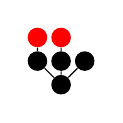
\begin{tikzpicture}[scale=.2]
\node[circle, scale=0.75, fill] (tid0) at (2.25,0){};
\node[circle, scale=0.75, fill] (tid1) at (0.75,1.5){};
\node[circle, scale=0.75, fill, red] (tid4) at (0.75,3){};
\draw[](tid1) -- (tid4);
\node[circle, scale=0.75, fill] (tid2) at (2.25,1.5){};
\node[circle, scale=0.75, fill, red] (tid5) at (2.25,3){};
\draw[](tid2) -- (tid5);
\node[circle, scale=0.75, fill] (tid3) at (3.75,1.5){};
\draw[](tid0) -- (tid1);
\draw[](tid0) -- (tid2);
\draw[](tid0) -- (tid3);

\end{tikzpicture}
\nodepart{two}
\footnotesize{4.125}
};
\node[draw=black, rectangle split, rectangle split parts=2] (sn0x93ca478W-3) at (-3.25, -72) {
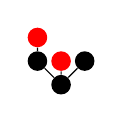
\begin{tikzpicture}[scale=.2]
\node[circle, scale=0.75, fill] (tid0) at (2.25,0){};
\node[circle, scale=0.75, fill] (tid1) at (0.75,1.5){};
\node[circle, scale=0.75, fill, red] (tid4) at (0.75,3){};
\draw[](tid1) -- (tid4);
\node[circle, scale=0.75, fill, red] (tid2) at (2.25,1.5){};
\node[circle, scale=0.75, fill] (tid3) at (3.75,1.5){};
\draw[](tid0) -- (tid1);
\draw[](tid0) -- (tid2);
\draw[](tid0) -- (tid3);

\end{tikzpicture}
\nodepart{two}
\footnotesize{3.625}
};
\node[draw=black, rectangle split, rectangle split parts=2] (sn0x93ca4e0W-5) at (-5.75, -84) {
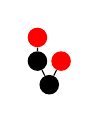
\begin{tikzpicture}[scale=.2]
\node[circle, scale=0.75, fill] (tid0) at (1.5,0){};
\node[circle, scale=0.75, fill] (tid1) at (0.75,1.5){};
\node[circle, scale=0.75, fill, red] (tid3) at (0.75,3){};
\draw[](tid1) -- (tid3);
\node[circle, scale=0.75, fill, red] (tid2) at (2.25,1.5){};
\draw[](tid0) -- (tid1);
\draw[](tid0) -- (tid2);

\end{tikzpicture}
\nodepart{two}
\footnotesize{3.25}
};
\node[draw=black, rectangle split, rectangle split parts=2] (sn0x93d1938W-4) at (-4.25, -96) {
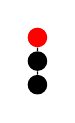
\begin{tikzpicture}[scale=.2]
\node[circle, scale=0.75, fill] (tid0) at (0.75,0){};
\node[circle, scale=0.75, fill] (tid1) at (0.75,1.5){};
\node[circle, scale=0.75, fill, red] (tid2) at (0.75,3){};
\draw[](tid1) -- (tid2);
\draw[](tid0) -- (tid1);

\end{tikzpicture}
\nodepart{two}
\footnotesize{3}
};
\node[draw=black, rectangle split, rectangle split parts=2] (sn0x93d1c08W-1) at (-1.75, -108) {

\begin{tikzpicture}[scale=.2]
\node[circle, scale=0.75, fill] (tid0) at (0.75,0){};
\node[circle, scale=0.75, fill, red] (tid1) at (0.75,1.5){};
\draw[](tid0) -- (tid1);

\end{tikzpicture}
\nodepart{two}
\footnotesize{2}
};
\draw (sn0x93d1938W-4.south) -- (sn0x93d1c08W-1.north);
\node[draw=black, rectangle split, rectangle split parts=2] (sn0x93d1a28W0) at (-0.75, -96) {

\begin{tikzpicture}[scale=.2]
\node[circle, scale=0.75, fill] (tid0) at (1.5,0){};
\node[circle, scale=0.75, fill, red] (tid1) at (0.75,1.5){};
\node[circle, scale=0.75, fill, red] (tid2) at (2.25,1.5){};
\draw[](tid0) -- (tid1);
\draw[](tid0) -- (tid2);

\end{tikzpicture}
\nodepart{two}
\footnotesize{2.5}
};
\draw (sn0x93d1a28W0.south) -- (sn0x93d1c08W-1.north);
\draw (sn0x93ca4e0W-5.south) -- (sn0x93d1938W-4.north);
\draw (sn0x93ca4e0W-5.south) -- (sn0x93d1a28W0.north);
\node[draw=black, rectangle split, rectangle split parts=2] (sn0x93cab38W0) at (-0.75, -84) {
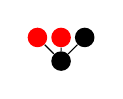
\begin{tikzpicture}[scale=.2]
\node[circle, scale=0.75, fill] (tid0) at (2.25,0){};
\node[circle, scale=0.75, fill, red] (tid1) at (0.75,1.5){};
\node[circle, scale=0.75, fill, red] (tid2) at (2.25,1.5){};
\node[circle, scale=0.75, fill] (tid3) at (3.75,1.5){};
\draw[](tid0) -- (tid1);
\draw[](tid0) -- (tid2);
\draw[](tid0) -- (tid3);

\end{tikzpicture}
\nodepart{two}
\footnotesize{3}
};
\draw (sn0x93cab38W0.south) -- (sn0x93d1a28W0.north);
\draw (sn0x93ca478W-3.south) -- (sn0x93ca4e0W-5.north);
\draw (sn0x93ca478W-3.south) -- (sn0x93cab38W0.north);
\draw (sn0x93cb870W-7.south) -- (sn0x93ca478W-3.north);
\node[draw=black, rectangle split, rectangle split parts=2] (sn0x93d2048W0) at (-0.75, -60) {
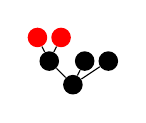
\begin{tikzpicture}[scale=.2]
\node[circle, scale=0.75, fill] (tid0) at (3,0){};
\node[circle, scale=0.75, fill] (tid1) at (1.5,1.5){};
\node[circle, scale=0.75, fill, red] (tid4) at (0.75,3){};
\node[circle, scale=0.75, fill, red] (tid5) at (2.25,3){};
\draw[](tid1) -- (tid4);
\draw[](tid1) -- (tid5);
\node[circle, scale=0.75, fill] (tid2) at (3.75,1.5){};
\node[circle, scale=0.75, fill] (tid3) at (5.25,1.5){};
\draw[](tid0) -- (tid1);
\draw[](tid0) -- (tid2);
\draw[](tid0) -- (tid3);

\end{tikzpicture}
\nodepart{two}
\footnotesize{4.125}
};
\draw (sn0x93d2048W0.south) -- (sn0x93ca478W-3.north);
\draw (sn0x93cb808W-19.south) -- (sn0x93cb870W-7.north);
\draw (sn0x93cb808W-19.south) -- (sn0x93d2048W0.north);
\draw (sn0x93c8a38W-31.south) -- (sn0x93cb808W-19.north);
\node[draw=black, rectangle split, rectangle split parts=2] (sn0x93d2868W-23) at (-23.75, -36) {
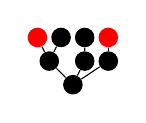
\begin{tikzpicture}[scale=.2]
\node[circle, scale=0.75, fill] (tid0) at (3,0){};
\node[circle, scale=0.75, fill] (tid1) at (1.5,1.5){};
\node[circle, scale=0.75, fill, red] (tid4) at (0.75,3){};
\node[circle, scale=0.75, fill] (tid5) at (2.25,3){};
\draw[](tid1) -- (tid4);
\draw[](tid1) -- (tid5);
\node[circle, scale=0.75, fill] (tid2) at (3.75,1.5){};
\node[circle, scale=0.75, fill] (tid6) at (3.75,3){};
\draw[](tid2) -- (tid6);
\node[circle, scale=0.75, fill] (tid3) at (5.25,1.5){};
\node[circle, scale=0.75, fill, red] (tid7) at (5.25,3){};
\draw[](tid3) -- (tid7);
\draw[](tid0) -- (tid1);
\draw[](tid0) -- (tid2);
\draw[](tid0) -- (tid3);

\end{tikzpicture}
\nodepart{two}
\footnotesize{5.125}
};
\node[draw=black, rectangle split, rectangle split parts=2] (sn0x93d2c08W-11) at (-11.25, -48) {
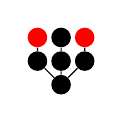
\begin{tikzpicture}[scale=.2]
\node[circle, scale=0.75, fill] (tid0) at (2.25,0){};
\node[circle, scale=0.75, fill] (tid1) at (0.75,1.5){};
\node[circle, scale=0.75, fill, red] (tid4) at (0.75,3){};
\draw[](tid1) -- (tid4);
\node[circle, scale=0.75, fill] (tid2) at (2.25,1.5){};
\node[circle, scale=0.75, fill] (tid5) at (2.25,3){};
\draw[](tid2) -- (tid5);
\node[circle, scale=0.75, fill] (tid3) at (3.75,1.5){};
\node[circle, scale=0.75, fill, red] (tid6) at (3.75,3){};
\draw[](tid3) -- (tid6);
\draw[](tid0) -- (tid1);
\draw[](tid0) -- (tid2);
\draw[](tid0) -- (tid3);

\end{tikzpicture}
\nodepart{two}
\footnotesize{4.625}
};
\draw (sn0x93d2c08W-11.south) -- (sn0x93cb870W-7.north);
\node[draw=black, rectangle split, rectangle split parts=2] (sn0x93cb048W-4) at (-4.75, -48) {
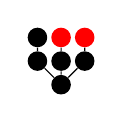
\begin{tikzpicture}[scale=.2]
\node[circle, scale=0.75, fill] (tid0) at (2.25,0){};
\node[circle, scale=0.75, fill] (tid1) at (0.75,1.5){};
\node[circle, scale=0.75, fill] (tid4) at (0.75,3){};
\draw[](tid1) -- (tid4);
\node[circle, scale=0.75, fill] (tid2) at (2.25,1.5){};
\node[circle, scale=0.75, fill, red] (tid5) at (2.25,3){};
\draw[](tid2) -- (tid5);
\node[circle, scale=0.75, fill] (tid3) at (3.75,1.5){};
\node[circle, scale=0.75, fill, red] (tid6) at (3.75,3){};
\draw[](tid3) -- (tid6);
\draw[](tid0) -- (tid1);
\draw[](tid0) -- (tid2);
\draw[](tid0) -- (tid3);

\end{tikzpicture}
\nodepart{two}
\footnotesize{4.625}
};
\draw (sn0x93cb048W-4.south) -- (sn0x93cb870W-7.north);
\node[draw=black, rectangle split, rectangle split parts=2] (sn0x93ca858W1) at (1.75, -48) {
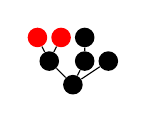
\begin{tikzpicture}[scale=.2]
\node[circle, scale=0.75, fill] (tid0) at (3,0){};
\node[circle, scale=0.75, fill] (tid1) at (1.5,1.5){};
\node[circle, scale=0.75, fill, red] (tid4) at (0.75,3){};
\node[circle, scale=0.75, fill, red] (tid5) at (2.25,3){};
\draw[](tid1) -- (tid4);
\draw[](tid1) -- (tid5);
\node[circle, scale=0.75, fill] (tid2) at (3.75,1.5){};
\node[circle, scale=0.75, fill] (tid6) at (3.75,3){};
\draw[](tid2) -- (tid6);
\node[circle, scale=0.75, fill] (tid3) at (5.25,1.5){};
\draw[](tid0) -- (tid1);
\draw[](tid0) -- (tid2);
\draw[](tid0) -- (tid3);

\end{tikzpicture}
\nodepart{two}
\footnotesize{4.625}
};
\draw (sn0x93ca858W1.south) -- (sn0x93cb870W-7.north);
\draw (sn0x93d2868W-23.south) -- (sn0x93d2c08W-11.north);
\draw (sn0x93d2868W-23.south) -- (sn0x93cb048W-4.north);
\draw (sn0x93d2868W-23.south) -- (sn0x93ca858W1.north);
\draw (sn0x93d2868W-23.south) -- (sn0x93cb808W-19.north);
\node[draw=black, rectangle split, rectangle split parts=2] (sn0x93d2dc8W-15) at (-15.75, -36) {
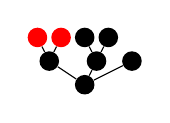
\begin{tikzpicture}[scale=.2]
\node[circle, scale=0.75, fill] (tid0) at (3.75,0){};
\node[circle, scale=0.75, fill] (tid1) at (1.5,1.5){};
\node[circle, scale=0.75, fill, red] (tid4) at (0.75,3){};
\node[circle, scale=0.75, fill, red] (tid5) at (2.25,3){};
\draw[](tid1) -- (tid4);
\draw[](tid1) -- (tid5);
\node[circle, scale=0.75, fill] (tid2) at (4.5,1.5){};
\node[circle, scale=0.75, fill] (tid6) at (3.75,3){};
\node[circle, scale=0.75, fill] (tid7) at (5.25,3){};
\draw[](tid2) -- (tid6);
\draw[](tid2) -- (tid7);
\node[circle, scale=0.75, fill] (tid3) at (6.75,1.5){};
\draw[](tid0) -- (tid1);
\draw[](tid0) -- (tid2);
\draw[](tid0) -- (tid3);

\end{tikzpicture}
\nodepart{two}
\footnotesize{5.125}
};
\draw (sn0x93d2dc8W-15.south) -- (sn0x93cb808W-19.north);
\node[draw=black, rectangle split, rectangle split parts=2] (sn0x93d2e60W-6) at (-6.25, -36) {
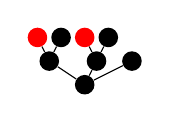
\begin{tikzpicture}[scale=.2]
\node[circle, scale=0.75, fill] (tid0) at (3.75,0){};
\node[circle, scale=0.75, fill] (tid1) at (1.5,1.5){};
\node[circle, scale=0.75, fill, red] (tid4) at (0.75,3){};
\node[circle, scale=0.75, fill] (tid5) at (2.25,3){};
\draw[](tid1) -- (tid4);
\draw[](tid1) -- (tid5);
\node[circle, scale=0.75, fill] (tid2) at (4.5,1.5){};
\node[circle, scale=0.75, fill, red] (tid6) at (3.75,3){};
\node[circle, scale=0.75, fill] (tid7) at (5.25,3){};
\draw[](tid2) -- (tid6);
\draw[](tid2) -- (tid7);
\node[circle, scale=0.75, fill] (tid3) at (6.75,1.5){};
\draw[](tid0) -- (tid1);
\draw[](tid0) -- (tid2);
\draw[](tid0) -- (tid3);

\end{tikzpicture}
\nodepart{two}
\footnotesize{5.125}
};
\draw (sn0x93d2e60W-6.south) -- (sn0x93cb808W-19.north);
\draw (sn0x93d2e60W-6.south) -- (sn0x93ca858W1.north);
\draw (sn0x93c90c8W-20.south) -- (sn0x93c8a38W-31.north);
\draw (sn0x93c90c8W-20.south) -- (sn0x93d2868W-23.north);
\draw (sn0x93c90c8W-20.south) -- (sn0x93d2dc8W-15.north);
\draw (sn0x93c90c8W-20.south) -- (sn0x93d2e60W-6.north);
\node[draw=black, rectangle split, rectangle split parts=2] (sn0x93d3218W-11) at (-11, -24) {
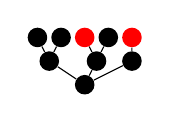
\begin{tikzpicture}[scale=.2]
\node[circle, scale=0.75, fill] (tid0) at (3.75,0){};
\node[circle, scale=0.75, fill] (tid1) at (1.5,1.5){};
\node[circle, scale=0.75, fill] (tid4) at (0.75,3){};
\node[circle, scale=0.75, fill] (tid5) at (2.25,3){};
\draw[](tid1) -- (tid4);
\draw[](tid1) -- (tid5);
\node[circle, scale=0.75, fill] (tid2) at (4.5,1.5){};
\node[circle, scale=0.75, fill, red] (tid6) at (3.75,3){};
\node[circle, scale=0.75, fill] (tid7) at (5.25,3){};
\draw[](tid2) -- (tid6);
\draw[](tid2) -- (tid7);
\node[circle, scale=0.75, fill] (tid3) at (6.75,1.5){};
\node[circle, scale=0.75, fill, red] (tid8) at (6.75,3){};
\draw[](tid3) -- (tid8);
\draw[](tid0) -- (tid1);
\draw[](tid0) -- (tid2);
\draw[](tid0) -- (tid3);

\end{tikzpicture}
\nodepart{two}
\footnotesize{5.625}
};
\node[draw=black, rectangle split, rectangle split parts=2] (sn0x93d3d88W3) at (3.25, -36) {
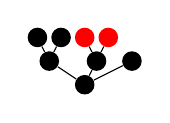
\begin{tikzpicture}[scale=.2]
\node[circle, scale=0.75, fill] (tid0) at (3.75,0){};
\node[circle, scale=0.75, fill] (tid1) at (1.5,1.5){};
\node[circle, scale=0.75, fill] (tid4) at (0.75,3){};
\node[circle, scale=0.75, fill] (tid5) at (2.25,3){};
\draw[](tid1) -- (tid4);
\draw[](tid1) -- (tid5);
\node[circle, scale=0.75, fill] (tid2) at (4.5,1.5){};
\node[circle, scale=0.75, fill, red] (tid6) at (3.75,3){};
\node[circle, scale=0.75, fill, red] (tid7) at (5.25,3){};
\draw[](tid2) -- (tid6);
\draw[](tid2) -- (tid7);
\node[circle, scale=0.75, fill] (tid3) at (6.75,1.5){};
\draw[](tid0) -- (tid1);
\draw[](tid0) -- (tid2);
\draw[](tid0) -- (tid3);

\end{tikzpicture}
\nodepart{two}
\footnotesize{5.125}
};
\draw (sn0x93d3d88W3.south) -- (sn0x93cb808W-19.north);
\draw (sn0x93d3218W-11.south) -- (sn0x93d2868W-23.north);
\draw (sn0x93d3218W-11.south) -- (sn0x93c8a38W-31.north);
\draw (sn0x93d3218W-11.south) -- (sn0x93d2e60W-6.north);
\draw (sn0x93d3218W-11.south) -- (sn0x93d3d88W3.north);
\node[draw=black, rectangle split, rectangle split parts=2] (sn0x93d3b60W-1) at (-1.5, -24) {
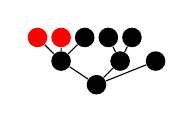
\begin{tikzpicture}[scale=.2]
\node[circle, scale=0.75, fill] (tid0) at (4.5,0){};
\node[circle, scale=0.75, fill] (tid1) at (2.25,1.5){};
\node[circle, scale=0.75, fill, red] (tid4) at (0.75,3){};
\node[circle, scale=0.75, fill, red] (tid5) at (2.25,3){};
\node[circle, scale=0.75, fill] (tid6) at (3.75,3){};
\draw[](tid1) -- (tid4);
\draw[](tid1) -- (tid5);
\draw[](tid1) -- (tid6);
\node[circle, scale=0.75, fill] (tid2) at (6,1.5){};
\node[circle, scale=0.75, fill] (tid7) at (5.25,3){};
\node[circle, scale=0.75, fill] (tid8) at (6.75,3){};
\draw[](tid2) -- (tid7);
\draw[](tid2) -- (tid8);
\node[circle, scale=0.75, fill] (tid3) at (8.25,1.5){};
\draw[](tid0) -- (tid1);
\draw[](tid0) -- (tid2);
\draw[](tid0) -- (tid3);

\end{tikzpicture}
\nodepart{two}
\footnotesize{5.625}
};
\draw (sn0x93d3b60W-1.south) -- (sn0x93d2dc8W-15.north);
\draw (sn0x93d3b60W-1.south) -- (sn0x93d2e60W-6.north);
\node[draw=black, rectangle split, rectangle split parts=2] (sn0x93d36b8W9) at (9.5, -24) {
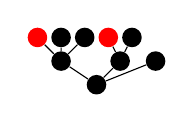
\begin{tikzpicture}[scale=.2]
\node[circle, scale=0.75, fill] (tid0) at (4.5,0){};
\node[circle, scale=0.75, fill] (tid1) at (2.25,1.5){};
\node[circle, scale=0.75, fill, red] (tid4) at (0.75,3){};
\node[circle, scale=0.75, fill] (tid5) at (2.25,3){};
\node[circle, scale=0.75, fill] (tid6) at (3.75,3){};
\draw[](tid1) -- (tid4);
\draw[](tid1) -- (tid5);
\draw[](tid1) -- (tid6);
\node[circle, scale=0.75, fill] (tid2) at (6,1.5){};
\node[circle, scale=0.75, fill, red] (tid7) at (5.25,3){};
\node[circle, scale=0.75, fill] (tid8) at (6.75,3){};
\draw[](tid2) -- (tid7);
\draw[](tid2) -- (tid8);
\node[circle, scale=0.75, fill] (tid3) at (8.25,1.5){};
\draw[](tid0) -- (tid1);
\draw[](tid0) -- (tid2);
\draw[](tid0) -- (tid3);

\end{tikzpicture}
\nodepart{two}
\footnotesize{5.625}
};
\node[draw=black, rectangle split, rectangle split parts=2] (sn0x93d38b8W12) at (12.75, -36) {
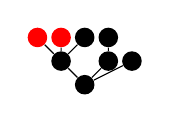
\begin{tikzpicture}[scale=.2]
\node[circle, scale=0.75, fill] (tid0) at (3.75,0){};
\node[circle, scale=0.75, fill] (tid1) at (2.25,1.5){};
\node[circle, scale=0.75, fill, red] (tid4) at (0.75,3){};
\node[circle, scale=0.75, fill, red] (tid5) at (2.25,3){};
\node[circle, scale=0.75, fill] (tid6) at (3.75,3){};
\draw[](tid1) -- (tid4);
\draw[](tid1) -- (tid5);
\draw[](tid1) -- (tid6);
\node[circle, scale=0.75, fill] (tid2) at (5.25,1.5){};
\node[circle, scale=0.75, fill] (tid7) at (5.25,3){};
\draw[](tid2) -- (tid7);
\node[circle, scale=0.75, fill] (tid3) at (6.75,1.5){};
\draw[](tid0) -- (tid1);
\draw[](tid0) -- (tid2);
\draw[](tid0) -- (tid3);

\end{tikzpicture}
\nodepart{two}
\footnotesize{5.125}
};
\draw (sn0x93d38b8W12.south) -- (sn0x93ca858W1.north);
\draw (sn0x93d38b8W12.south) -- (sn0x93cb808W-19.north);
\node[draw=black, rectangle split, rectangle split parts=2] (sn0x93d44a0W22) at (22.25, -36) {
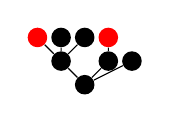
\begin{tikzpicture}[scale=.2]
\node[circle, scale=0.75, fill] (tid0) at (3.75,0){};
\node[circle, scale=0.75, fill] (tid1) at (2.25,1.5){};
\node[circle, scale=0.75, fill, red] (tid4) at (0.75,3){};
\node[circle, scale=0.75, fill] (tid5) at (2.25,3){};
\node[circle, scale=0.75, fill] (tid6) at (3.75,3){};
\draw[](tid1) -- (tid4);
\draw[](tid1) -- (tid5);
\draw[](tid1) -- (tid6);
\node[circle, scale=0.75, fill] (tid2) at (5.25,1.5){};
\node[circle, scale=0.75, fill, red] (tid7) at (5.25,3){};
\draw[](tid2) -- (tid7);
\node[circle, scale=0.75, fill] (tid3) at (6.75,1.5){};
\draw[](tid0) -- (tid1);
\draw[](tid0) -- (tid2);
\draw[](tid0) -- (tid3);

\end{tikzpicture}
\nodepart{two}
\footnotesize{5.125}
};
\node[draw=black, rectangle split, rectangle split parts=2] (sn0x93d4c20W9) at (9.75, -48) {
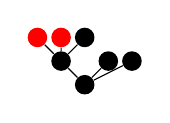
\begin{tikzpicture}[scale=.2]
\node[circle, scale=0.75, fill] (tid0) at (3.75,0){};
\node[circle, scale=0.75, fill] (tid1) at (2.25,1.5){};
\node[circle, scale=0.75, fill, red] (tid4) at (0.75,3){};
\node[circle, scale=0.75, fill, red] (tid5) at (2.25,3){};
\node[circle, scale=0.75, fill] (tid6) at (3.75,3){};
\draw[](tid1) -- (tid4);
\draw[](tid1) -- (tid5);
\draw[](tid1) -- (tid6);
\node[circle, scale=0.75, fill] (tid2) at (5.25,1.5){};
\node[circle, scale=0.75, fill] (tid3) at (6.75,1.5){};
\draw[](tid0) -- (tid1);
\draw[](tid0) -- (tid2);
\draw[](tid0) -- (tid3);

\end{tikzpicture}
\nodepart{two}
\footnotesize{4.625}
};
\draw (sn0x93d4c20W9.south) -- (sn0x93d2048W0.north);
\draw (sn0x93d44a0W22.south) -- (sn0x93cb808W-19.north);
\draw (sn0x93d44a0W22.south) -- (sn0x93d4c20W9.north);
\draw (sn0x93d36b8W9.south) -- (sn0x93d2e60W-6.north);
\draw (sn0x93d36b8W9.south) -- (sn0x93d3d88W3.north);
\draw (sn0x93d36b8W9.south) -- (sn0x93d38b8W12.north);
\draw (sn0x93d36b8W9.south) -- (sn0x93d44a0W22.north);
\draw (sn0x93c9ba0W-5.south) -- (sn0x93c90c8W-20.north);
\draw (sn0x93c9ba0W-5.south) -- (sn0x93d3218W-11.north);
\draw (sn0x93c9ba0W-5.south) -- (sn0x93d3b60W-1.north);
\draw (sn0x93c9ba0W-5.south) -- (sn0x93d36b8W9.north);
\end{tikzpicture}

%%% Local Variables:
%%% TeX-master: "thesis/thesis.tex"
%%% End: 

\begin{tikzpicture}[scale=.2, anchor=south west]
\node[draw=black, rectangle split, rectangle split parts=2] (sn0x93c9c00W-5) at (-5.5, -12) {
\begin{tikzpicture}[scale=.2]
\node[circle, scale=0.75, fill] (tid0) at (4.5,0){};
\node[circle, scale=0.75, fill] (tid1) at (2.25,1.5){};
\node[circle, scale=0.75, fill, red] (tid4) at (0.75,3){};
\node[circle, scale=0.75, fill] (tid5) at (2.25,3){};
\node[circle, scale=0.75, fill] (tid6) at (3.75,3){};
\draw[](tid1) -- (tid4);
\draw[](tid1) -- (tid5);
\draw[](tid1) -- (tid6);
\node[circle, scale=0.75, fill] (tid2) at (6,1.5){};
\node[circle, scale=0.75, fill, red] (tid7) at (5.25,3){};
\node[circle, scale=0.75, fill] (tid8) at (6.75,3){};
\draw[](tid2) -- (tid7);
\draw[](tid2) -- (tid8);
\node[circle, scale=0.75, fill] (tid3) at (8.25,1.5){};
\node[circle, scale=0.75, fill] (tid9) at (8.25,3){};
\draw[](tid3) -- (tid9);
\draw[](tid0) -- (tid1);
\draw[](tid0) -- (tid2);
\draw[](tid0) -- (tid3);

\end{tikzpicture}
\nodepart{two}
\footnotesize{6.125}
};
\node[draw=black, rectangle split, rectangle split parts=2] (sn0x93c8458W-28) at (-28.5, -24) {
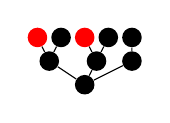
\begin{tikzpicture}[scale=.2]
\node[circle, scale=0.75, fill] (tid0) at (3.75,0){};
\node[circle, scale=0.75, fill] (tid1) at (1.5,1.5){};
\node[circle, scale=0.75, fill, red] (tid4) at (0.75,3){};
\node[circle, scale=0.75, fill] (tid5) at (2.25,3){};
\draw[](tid1) -- (tid4);
\draw[](tid1) -- (tid5);
\node[circle, scale=0.75, fill] (tid2) at (4.5,1.5){};
\node[circle, scale=0.75, fill, red] (tid6) at (3.75,3){};
\node[circle, scale=0.75, fill] (tid7) at (5.25,3){};
\draw[](tid2) -- (tid6);
\draw[](tid2) -- (tid7);
\node[circle, scale=0.75, fill] (tid3) at (6.75,1.5){};
\node[circle, scale=0.75, fill] (tid8) at (6.75,3){};
\draw[](tid3) -- (tid8);
\draw[](tid0) -- (tid1);
\draw[](tid0) -- (tid2);
\draw[](tid0) -- (tid3);

\end{tikzpicture}
\nodepart{two}
\footnotesize{5.625}
};
\node[draw=black, rectangle split, rectangle split parts=2] (sn0x93d1558W-35) at (-35, -36) {
\begin{tikzpicture}[scale=.2]
\node[circle, scale=0.75, fill] (tid0) at (3,0){};
\node[circle, scale=0.75, fill] (tid1) at (1.5,1.5){};
\node[circle, scale=0.75, fill, red] (tid4) at (0.75,3){};
\node[circle, scale=0.75, fill] (tid5) at (2.25,3){};
\draw[](tid1) -- (tid4);
\draw[](tid1) -- (tid5);
\node[circle, scale=0.75, fill] (tid2) at (3.75,1.5){};
\node[circle, scale=0.75, fill, red] (tid6) at (3.75,3){};
\draw[](tid2) -- (tid6);
\node[circle, scale=0.75, fill] (tid3) at (5.25,1.5){};
\node[circle, scale=0.75, fill] (tid7) at (5.25,3){};
\draw[](tid3) -- (tid7);
\draw[](tid0) -- (tid1);
\draw[](tid0) -- (tid2);
\draw[](tid0) -- (tid3);

\end{tikzpicture}
\nodepart{two}
\footnotesize{5.125}
};
\node[draw=black, rectangle split, rectangle split parts=2] (sn0x93d0fa8W-22) at (-22.5, -48) {
\begin{tikzpicture}[scale=.2]
\node[circle, scale=0.75, fill] (tid0) at (2.25,0){};
\node[circle, scale=0.75, fill] (tid1) at (0.75,1.5){};
\node[circle, scale=0.75, fill, red] (tid4) at (0.75,3){};
\draw[](tid1) -- (tid4);
\node[circle, scale=0.75, fill] (tid2) at (2.25,1.5){};
\node[circle, scale=0.75, fill, red] (tid5) at (2.25,3){};
\draw[](tid2) -- (tid5);
\node[circle, scale=0.75, fill] (tid3) at (3.75,1.5){};
\node[circle, scale=0.75, fill] (tid6) at (3.75,3){};
\draw[](tid3) -- (tid6);
\draw[](tid0) -- (tid1);
\draw[](tid0) -- (tid2);
\draw[](tid0) -- (tid3);

\end{tikzpicture}
\nodepart{two}
\footnotesize{4.625}
};
\node[draw=black, rectangle split, rectangle split parts=2] (sn0x93cb870W-7) at (-7.25, -60) {
\begin{tikzpicture}[scale=.2]
\node[circle, scale=0.75, fill] (tid0) at (2.25,0){};
\node[circle, scale=0.75, fill] (tid1) at (0.75,1.5){};
\node[circle, scale=0.75, fill, red] (tid4) at (0.75,3){};
\draw[](tid1) -- (tid4);
\node[circle, scale=0.75, fill] (tid2) at (2.25,1.5){};
\node[circle, scale=0.75, fill, red] (tid5) at (2.25,3){};
\draw[](tid2) -- (tid5);
\node[circle, scale=0.75, fill] (tid3) at (3.75,1.5){};
\draw[](tid0) -- (tid1);
\draw[](tid0) -- (tid2);
\draw[](tid0) -- (tid3);

\end{tikzpicture}
\nodepart{two}
\footnotesize{4.125}
};
\node[draw=black, rectangle split, rectangle split parts=2] (sn0x93ca478W-3) at (-3.25, -72) {
\begin{tikzpicture}[scale=.2]
\node[circle, scale=0.75, fill] (tid0) at (2.25,0){};
\node[circle, scale=0.75, fill] (tid1) at (0.75,1.5){};
\node[circle, scale=0.75, fill, red] (tid4) at (0.75,3){};
\draw[](tid1) -- (tid4);
\node[circle, scale=0.75, fill, red] (tid2) at (2.25,1.5){};
\node[circle, scale=0.75, fill] (tid3) at (3.75,1.5){};
\draw[](tid0) -- (tid1);
\draw[](tid0) -- (tid2);
\draw[](tid0) -- (tid3);

\end{tikzpicture}
\nodepart{two}
\footnotesize{3.625}
};
\node[draw=black, rectangle split, rectangle split parts=2] (sn0x93ca4e0W-5) at (-5.75, -84) {
\begin{tikzpicture}[scale=.2]
\node[circle, scale=0.75, fill] (tid0) at (1.5,0){};
\node[circle, scale=0.75, fill] (tid1) at (0.75,1.5){};
\node[circle, scale=0.75, fill, red] (tid3) at (0.75,3){};
\draw[](tid1) -- (tid3);
\node[circle, scale=0.75, fill, red] (tid2) at (2.25,1.5){};
\draw[](tid0) -- (tid1);
\draw[](tid0) -- (tid2);

\end{tikzpicture}
\nodepart{two}
\footnotesize{3.25}
};
\node[draw=black, rectangle split, rectangle split parts=2] (sn0x93d1938W-4) at (-4.25, -96) {
\begin{tikzpicture}[scale=.2]
\node[circle, scale=0.75, fill] (tid0) at (0.75,0){};
\node[circle, scale=0.75, fill] (tid1) at (0.75,1.5){};
\node[circle, scale=0.75, fill, red] (tid2) at (0.75,3){};
\draw[](tid1) -- (tid2);
\draw[](tid0) -- (tid1);

\end{tikzpicture}
\nodepart{two}
\footnotesize{3}
};
\node[draw=black, rectangle split, rectangle split parts=2] (sn0x93d1c08W-1) at (-1.75, -108) {
\begin{tikzpicture}[scale=.2]
\node[circle, scale=0.75, fill] (tid0) at (0.75,0){};
\node[circle, scale=0.75, fill, red] (tid1) at (0.75,1.5){};
\draw[](tid0) -- (tid1);

\end{tikzpicture}
\nodepart{two}
\footnotesize{2}
};
\draw (sn0x93d1938W-4.south) -- (sn0x93d1c08W-1.north);
\node[draw=black, rectangle split, rectangle split parts=2] (sn0x93d1a28W0) at (-0.75, -96) {
\begin{tikzpicture}[scale=.2]
\node[circle, scale=0.75, fill] (tid0) at (1.5,0){};
\node[circle, scale=0.75, fill, red] (tid1) at (0.75,1.5){};
\node[circle, scale=0.75, fill, red] (tid2) at (2.25,1.5){};
\draw[](tid0) -- (tid1);
\draw[](tid0) -- (tid2);

\end{tikzpicture}
\nodepart{two}
\footnotesize{2.5}
};
\draw (sn0x93d1a28W0.south) -- (sn0x93d1c08W-1.north);
\draw (sn0x93ca4e0W-5.south) -- (sn0x93d1938W-4.north);
\draw (sn0x93ca4e0W-5.south) -- (sn0x93d1a28W0.north);
\node[draw=black, rectangle split, rectangle split parts=2] (sn0x93cab38W0) at (-0.75, -84) {
\begin{tikzpicture}[scale=.2]
\node[circle, scale=0.75, fill] (tid0) at (2.25,0){};
\node[circle, scale=0.75, fill, red] (tid1) at (0.75,1.5){};
\node[circle, scale=0.75, fill, red] (tid2) at (2.25,1.5){};
\node[circle, scale=0.75, fill] (tid3) at (3.75,1.5){};
\draw[](tid0) -- (tid1);
\draw[](tid0) -- (tid2);
\draw[](tid0) -- (tid3);

\end{tikzpicture}
\nodepart{two}
\footnotesize{3}
};
\draw (sn0x93cab38W0.south) -- (sn0x93d1a28W0.north);
\draw (sn0x93ca478W-3.south) -- (sn0x93ca4e0W-5.north);
\draw (sn0x93ca478W-3.south) -- (sn0x93cab38W0.north);
\draw (sn0x93cb870W-7.south) -- (sn0x93ca478W-3.north);
\draw (sn0x93d0fa8W-22.south) -- (sn0x93cb870W-7.north);
\node[draw=black, rectangle split, rectangle split parts=2] (sn0x93cb048W-16) at (-16, -48) {
\begin{tikzpicture}[scale=.2]
\node[circle, scale=0.75, fill] (tid0) at (2.25,0){};
\node[circle, scale=0.75, fill] (tid1) at (0.75,1.5){};
\node[circle, scale=0.75, fill] (tid4) at (0.75,3){};
\draw[](tid1) -- (tid4);
\node[circle, scale=0.75, fill] (tid2) at (2.25,1.5){};
\node[circle, scale=0.75, fill, red] (tid5) at (2.25,3){};
\draw[](tid2) -- (tid5);
\node[circle, scale=0.75, fill] (tid3) at (3.75,1.5){};
\node[circle, scale=0.75, fill, red] (tid6) at (3.75,3){};
\draw[](tid3) -- (tid6);
\draw[](tid0) -- (tid1);
\draw[](tid0) -- (tid2);
\draw[](tid0) -- (tid3);

\end{tikzpicture}
\nodepart{two}
\footnotesize{4.625}
};
\draw (sn0x93cb048W-16.south) -- (sn0x93cb870W-7.north);
\node[draw=black, rectangle split, rectangle split parts=2] (sn0x93ca858W-9) at (-9.5, -48) {
\begin{tikzpicture}[scale=.2]
\node[circle, scale=0.75, fill] (tid0) at (3,0){};
\node[circle, scale=0.75, fill] (tid1) at (1.5,1.5){};
\node[circle, scale=0.75, fill, red] (tid4) at (0.75,3){};
\node[circle, scale=0.75, fill, red] (tid5) at (2.25,3){};
\draw[](tid1) -- (tid4);
\draw[](tid1) -- (tid5);
\node[circle, scale=0.75, fill] (tid2) at (3.75,1.5){};
\node[circle, scale=0.75, fill] (tid6) at (3.75,3){};
\draw[](tid2) -- (tid6);
\node[circle, scale=0.75, fill] (tid3) at (5.25,1.5){};
\draw[](tid0) -- (tid1);
\draw[](tid0) -- (tid2);
\draw[](tid0) -- (tid3);

\end{tikzpicture}
\nodepart{two}
\footnotesize{4.625}
};
\draw (sn0x93ca858W-9.south) -- (sn0x93cb870W-7.north);
\node[draw=black, rectangle split, rectangle split parts=2] (sn0x93cb808W-1) at (-1.5, -48) {
\begin{tikzpicture}[scale=.2]
\node[circle, scale=0.75, fill] (tid0) at (3,0){};
\node[circle, scale=0.75, fill] (tid1) at (1.5,1.5){};
\node[circle, scale=0.75, fill, red] (tid4) at (0.75,3){};
\node[circle, scale=0.75, fill] (tid5) at (2.25,3){};
\draw[](tid1) -- (tid4);
\draw[](tid1) -- (tid5);
\node[circle, scale=0.75, fill] (tid2) at (3.75,1.5){};
\node[circle, scale=0.75, fill, red] (tid6) at (3.75,3){};
\draw[](tid2) -- (tid6);
\node[circle, scale=0.75, fill] (tid3) at (5.25,1.5){};
\draw[](tid0) -- (tid1);
\draw[](tid0) -- (tid2);
\draw[](tid0) -- (tid3);

\end{tikzpicture}
\nodepart{two}
\footnotesize{4.625}
};
\node[draw=black, rectangle split, rectangle split parts=2] (sn0x93d2048W0) at (-0.75, -60) {
\begin{tikzpicture}[scale=.2]
\node[circle, scale=0.75, fill] (tid0) at (3,0){};
\node[circle, scale=0.75, fill] (tid1) at (1.5,1.5){};
\node[circle, scale=0.75, fill, red] (tid4) at (0.75,3){};
\node[circle, scale=0.75, fill, red] (tid5) at (2.25,3){};
\draw[](tid1) -- (tid4);
\draw[](tid1) -- (tid5);
\node[circle, scale=0.75, fill] (tid2) at (3.75,1.5){};
\node[circle, scale=0.75, fill] (tid3) at (5.25,1.5){};
\draw[](tid0) -- (tid1);
\draw[](tid0) -- (tid2);
\draw[](tid0) -- (tid3);

\end{tikzpicture}
\nodepart{two}
\footnotesize{4.125}
};
\draw (sn0x93d2048W0.south) -- (sn0x93ca478W-3.north);
\draw (sn0x93cb808W-1.south) -- (sn0x93cb870W-7.north);
\draw (sn0x93cb808W-1.south) -- (sn0x93d2048W0.north);
\draw (sn0x93d1558W-35.south) -- (sn0x93d0fa8W-22.north);
\draw (sn0x93d1558W-35.south) -- (sn0x93cb048W-16.north);
\draw (sn0x93d1558W-35.south) -- (sn0x93ca858W-9.north);
\draw (sn0x93d1558W-35.south) -- (sn0x93cb808W-1.north);
\node[draw=black, rectangle split, rectangle split parts=2] (sn0x93d2660W-27) at (-27, -36) {
\begin{tikzpicture}[scale=.2]
\node[circle, scale=0.75, fill] (tid0) at (3,0){};
\node[circle, scale=0.75, fill] (tid1) at (1.5,1.5){};
\node[circle, scale=0.75, fill, red] (tid4) at (0.75,3){};
\node[circle, scale=0.75, fill, red] (tid5) at (2.25,3){};
\draw[](tid1) -- (tid4);
\draw[](tid1) -- (tid5);
\node[circle, scale=0.75, fill] (tid2) at (3.75,1.5){};
\node[circle, scale=0.75, fill] (tid6) at (3.75,3){};
\draw[](tid2) -- (tid6);
\node[circle, scale=0.75, fill] (tid3) at (5.25,1.5){};
\node[circle, scale=0.75, fill] (tid7) at (5.25,3){};
\draw[](tid3) -- (tid7);
\draw[](tid0) -- (tid1);
\draw[](tid0) -- (tid2);
\draw[](tid0) -- (tid3);

\end{tikzpicture}
\nodepart{two}
\footnotesize{5.125}
};
\node[draw=black, rectangle split, rectangle split parts=2] (sn0x93d2c08W6) at (6.5, -48) {
\begin{tikzpicture}[scale=.2]
\node[circle, scale=0.75, fill] (tid0) at (2.25,0){};
\node[circle, scale=0.75, fill] (tid1) at (0.75,1.5){};
\node[circle, scale=0.75, fill, red] (tid4) at (0.75,3){};
\draw[](tid1) -- (tid4);
\node[circle, scale=0.75, fill] (tid2) at (2.25,1.5){};
\node[circle, scale=0.75, fill] (tid5) at (2.25,3){};
\draw[](tid2) -- (tid5);
\node[circle, scale=0.75, fill] (tid3) at (3.75,1.5){};
\node[circle, scale=0.75, fill, red] (tid6) at (3.75,3){};
\draw[](tid3) -- (tid6);
\draw[](tid0) -- (tid1);
\draw[](tid0) -- (tid2);
\draw[](tid0) -- (tid3);

\end{tikzpicture}
\nodepart{two}
\footnotesize{4.625}
};
\draw (sn0x93d2c08W6.south) -- (sn0x93cb870W-7.north);
\draw (sn0x93d2660W-27.south) -- (sn0x93d0fa8W-22.north);
\draw (sn0x93d2660W-27.south) -- (sn0x93d2c08W6.north);
\node[draw=black, rectangle split, rectangle split parts=2] (sn0x93d2868W-19) at (-19, -36) {
\begin{tikzpicture}[scale=.2]
\node[circle, scale=0.75, fill] (tid0) at (3,0){};
\node[circle, scale=0.75, fill] (tid1) at (1.5,1.5){};
\node[circle, scale=0.75, fill, red] (tid4) at (0.75,3){};
\node[circle, scale=0.75, fill] (tid5) at (2.25,3){};
\draw[](tid1) -- (tid4);
\draw[](tid1) -- (tid5);
\node[circle, scale=0.75, fill] (tid2) at (3.75,1.5){};
\node[circle, scale=0.75, fill] (tid6) at (3.75,3){};
\draw[](tid2) -- (tid6);
\node[circle, scale=0.75, fill] (tid3) at (5.25,1.5){};
\node[circle, scale=0.75, fill, red] (tid7) at (5.25,3){};
\draw[](tid3) -- (tid7);
\draw[](tid0) -- (tid1);
\draw[](tid0) -- (tid2);
\draw[](tid0) -- (tid3);

\end{tikzpicture}
\nodepart{two}
\footnotesize{5.125}
};
\draw (sn0x93d2868W-19.south) -- (sn0x93d2c08W6.north);
\draw (sn0x93d2868W-19.south) -- (sn0x93cb048W-16.north);
\draw (sn0x93d2868W-19.south) -- (sn0x93ca858W-9.north);
\draw (sn0x93d2868W-19.south) -- (sn0x93cb808W-1.north);
\draw (sn0x93c8458W-28.south) -- (sn0x93d1558W-35.north);
\draw (sn0x93c8458W-28.south) -- (sn0x93d2660W-27.north);
\draw (sn0x93c8458W-28.south) -- (sn0x93d2868W-19.north);
\node[draw=black, rectangle split, rectangle split parts=2] (sn0x93d4dc0W-19) at (-19, -24) {
\begin{tikzpicture}[scale=.2]
\node[circle, scale=0.75, fill] (tid0) at (3.75,0){};
\node[circle, scale=0.75, fill] (tid1) at (1.5,1.5){};
\node[circle, scale=0.75, fill] (tid4) at (0.75,3){};
\node[circle, scale=0.75, fill] (tid5) at (2.25,3){};
\draw[](tid1) -- (tid4);
\draw[](tid1) -- (tid5);
\node[circle, scale=0.75, fill] (tid2) at (4.5,1.5){};
\node[circle, scale=0.75, fill, red] (tid6) at (3.75,3){};
\node[circle, scale=0.75, fill, red] (tid7) at (5.25,3){};
\draw[](tid2) -- (tid6);
\draw[](tid2) -- (tid7);
\node[circle, scale=0.75, fill] (tid3) at (6.75,1.5){};
\node[circle, scale=0.75, fill] (tid8) at (6.75,3){};
\draw[](tid3) -- (tid8);
\draw[](tid0) -- (tid1);
\draw[](tid0) -- (tid2);
\draw[](tid0) -- (tid3);

\end{tikzpicture}
\nodepart{two}
\footnotesize{5.625}
};
\node[draw=black, rectangle split, rectangle split parts=2] (sn0x93c8a38W-11) at (-11, -36) {
\begin{tikzpicture}[scale=.2]
\node[circle, scale=0.75, fill] (tid0) at (3,0){};
\node[circle, scale=0.75, fill] (tid1) at (1.5,1.5){};
\node[circle, scale=0.75, fill] (tid4) at (0.75,3){};
\node[circle, scale=0.75, fill] (tid5) at (2.25,3){};
\draw[](tid1) -- (tid4);
\draw[](tid1) -- (tid5);
\node[circle, scale=0.75, fill] (tid2) at (3.75,1.5){};
\node[circle, scale=0.75, fill, red] (tid6) at (3.75,3){};
\draw[](tid2) -- (tid6);
\node[circle, scale=0.75, fill] (tid3) at (5.25,1.5){};
\node[circle, scale=0.75, fill, red] (tid7) at (5.25,3){};
\draw[](tid3) -- (tid7);
\draw[](tid0) -- (tid1);
\draw[](tid0) -- (tid2);
\draw[](tid0) -- (tid3);

\end{tikzpicture}
\nodepart{two}
\footnotesize{5.125}
};
\draw (sn0x93c8a38W-11.south) -- (sn0x93cb808W-1.north);
\draw (sn0x93d4dc0W-19.south) -- (sn0x93d1558W-35.north);
\draw (sn0x93d4dc0W-19.south) -- (sn0x93c8a38W-11.north);
\node[draw=black, rectangle split, rectangle split parts=2] (sn0x93d3218W-9) at (-9.5, -24) {
\begin{tikzpicture}[scale=.2]
\node[circle, scale=0.75, fill] (tid0) at (3.75,0){};
\node[circle, scale=0.75, fill] (tid1) at (1.5,1.5){};
\node[circle, scale=0.75, fill] (tid4) at (0.75,3){};
\node[circle, scale=0.75, fill] (tid5) at (2.25,3){};
\draw[](tid1) -- (tid4);
\draw[](tid1) -- (tid5);
\node[circle, scale=0.75, fill] (tid2) at (4.5,1.5){};
\node[circle, scale=0.75, fill, red] (tid6) at (3.75,3){};
\node[circle, scale=0.75, fill] (tid7) at (5.25,3){};
\draw[](tid2) -- (tid6);
\draw[](tid2) -- (tid7);
\node[circle, scale=0.75, fill] (tid3) at (6.75,1.5){};
\node[circle, scale=0.75, fill, red] (tid8) at (6.75,3){};
\draw[](tid3) -- (tid8);
\draw[](tid0) -- (tid1);
\draw[](tid0) -- (tid2);
\draw[](tid0) -- (tid3);

\end{tikzpicture}
\nodepart{two}
\footnotesize{5.625}
};
\node[draw=black, rectangle split, rectangle split parts=2] (sn0x93d2e60W-3) at (-3, -36) {
\begin{tikzpicture}[scale=.2]
\node[circle, scale=0.75, fill] (tid0) at (3.75,0){};
\node[circle, scale=0.75, fill] (tid1) at (1.5,1.5){};
\node[circle, scale=0.75, fill, red] (tid4) at (0.75,3){};
\node[circle, scale=0.75, fill] (tid5) at (2.25,3){};
\draw[](tid1) -- (tid4);
\draw[](tid1) -- (tid5);
\node[circle, scale=0.75, fill] (tid2) at (4.5,1.5){};
\node[circle, scale=0.75, fill, red] (tid6) at (3.75,3){};
\node[circle, scale=0.75, fill] (tid7) at (5.25,3){};
\draw[](tid2) -- (tid6);
\draw[](tid2) -- (tid7);
\node[circle, scale=0.75, fill] (tid3) at (6.75,1.5){};
\draw[](tid0) -- (tid1);
\draw[](tid0) -- (tid2);
\draw[](tid0) -- (tid3);

\end{tikzpicture}
\nodepart{two}
\footnotesize{5.125}
};
\draw (sn0x93d2e60W-3.south) -- (sn0x93cb808W-1.north);
\draw (sn0x93d2e60W-3.south) -- (sn0x93ca858W-9.north);
\node[draw=black, rectangle split, rectangle split parts=2] (sn0x93d3d88W6) at (6.5, -36) {
\begin{tikzpicture}[scale=.2]
\node[circle, scale=0.75, fill] (tid0) at (3.75,0){};
\node[circle, scale=0.75, fill] (tid1) at (1.5,1.5){};
\node[circle, scale=0.75, fill] (tid4) at (0.75,3){};
\node[circle, scale=0.75, fill] (tid5) at (2.25,3){};
\draw[](tid1) -- (tid4);
\draw[](tid1) -- (tid5);
\node[circle, scale=0.75, fill] (tid2) at (4.5,1.5){};
\node[circle, scale=0.75, fill, red] (tid6) at (3.75,3){};
\node[circle, scale=0.75, fill, red] (tid7) at (5.25,3){};
\draw[](tid2) -- (tid6);
\draw[](tid2) -- (tid7);
\node[circle, scale=0.75, fill] (tid3) at (6.75,1.5){};
\draw[](tid0) -- (tid1);
\draw[](tid0) -- (tid2);
\draw[](tid0) -- (tid3);

\end{tikzpicture}
\nodepart{two}
\footnotesize{5.125}
};
\draw (sn0x93d3d88W6.south) -- (sn0x93cb808W-1.north);
\draw (sn0x93d3218W-9.south) -- (sn0x93d2868W-19.north);
\draw (sn0x93d3218W-9.south) -- (sn0x93c8a38W-11.north);
\draw (sn0x93d3218W-9.south) -- (sn0x93d2e60W-3.north);
\draw (sn0x93d3218W-9.south) -- (sn0x93d3d88W6.north);
\node[draw=black, rectangle split, rectangle split parts=2] (sn0x93d4ce0W0) at (0, -24) {
\begin{tikzpicture}[scale=.2]
\node[circle, scale=0.75, fill] (tid0) at (3.75,0){};
\node[circle, scale=0.75, fill] (tid1) at (2.25,1.5){};
\node[circle, scale=0.75, fill, red] (tid4) at (0.75,3){};
\node[circle, scale=0.75, fill, red] (tid5) at (2.25,3){};
\node[circle, scale=0.75, fill] (tid6) at (3.75,3){};
\draw[](tid1) -- (tid4);
\draw[](tid1) -- (tid5);
\draw[](tid1) -- (tid6);
\node[circle, scale=0.75, fill] (tid2) at (5.25,1.5){};
\node[circle, scale=0.75, fill] (tid7) at (5.25,3){};
\draw[](tid2) -- (tid7);
\node[circle, scale=0.75, fill] (tid3) at (6.75,1.5){};
\node[circle, scale=0.75, fill] (tid8) at (6.75,3){};
\draw[](tid3) -- (tid8);
\draw[](tid0) -- (tid1);
\draw[](tid0) -- (tid2);
\draw[](tid0) -- (tid3);

\end{tikzpicture}
\nodepart{two}
\footnotesize{5.625}
};
\draw (sn0x93d4ce0W0.south) -- (sn0x93d2660W-27.north);
\draw (sn0x93d4ce0W0.south) -- (sn0x93d1558W-35.north);
\draw (sn0x93d4ce0W0.south) -- (sn0x93d2868W-19.north);
\node[draw=black, rectangle split, rectangle split parts=2] (sn0x93d54f0W9) at (9.5, -24) {
\begin{tikzpicture}[scale=.2]
\node[circle, scale=0.75, fill] (tid0) at (3.75,0){};
\node[circle, scale=0.75, fill] (tid1) at (2.25,1.5){};
\node[circle, scale=0.75, fill, red] (tid4) at (0.75,3){};
\node[circle, scale=0.75, fill] (tid5) at (2.25,3){};
\node[circle, scale=0.75, fill] (tid6) at (3.75,3){};
\draw[](tid1) -- (tid4);
\draw[](tid1) -- (tid5);
\draw[](tid1) -- (tid6);
\node[circle, scale=0.75, fill] (tid2) at (5.25,1.5){};
\node[circle, scale=0.75, fill, red] (tid7) at (5.25,3){};
\draw[](tid2) -- (tid7);
\node[circle, scale=0.75, fill] (tid3) at (6.75,1.5){};
\node[circle, scale=0.75, fill] (tid8) at (6.75,3){};
\draw[](tid3) -- (tid8);
\draw[](tid0) -- (tid1);
\draw[](tid0) -- (tid2);
\draw[](tid0) -- (tid3);

\end{tikzpicture}
\nodepart{two}
\footnotesize{5.625}
};
\node[draw=black, rectangle split, rectangle split parts=2] (sn0x93d38b8W16) at (16, -36) {
\begin{tikzpicture}[scale=.2]
\node[circle, scale=0.75, fill] (tid0) at (3.75,0){};
\node[circle, scale=0.75, fill] (tid1) at (2.25,1.5){};
\node[circle, scale=0.75, fill, red] (tid4) at (0.75,3){};
\node[circle, scale=0.75, fill, red] (tid5) at (2.25,3){};
\node[circle, scale=0.75, fill] (tid6) at (3.75,3){};
\draw[](tid1) -- (tid4);
\draw[](tid1) -- (tid5);
\draw[](tid1) -- (tid6);
\node[circle, scale=0.75, fill] (tid2) at (5.25,1.5){};
\node[circle, scale=0.75, fill] (tid7) at (5.25,3){};
\draw[](tid2) -- (tid7);
\node[circle, scale=0.75, fill] (tid3) at (6.75,1.5){};
\draw[](tid0) -- (tid1);
\draw[](tid0) -- (tid2);
\draw[](tid0) -- (tid3);

\end{tikzpicture}
\nodepart{two}
\footnotesize{5.125}
};
\draw (sn0x93d38b8W16.south) -- (sn0x93ca858W-9.north);
\draw (sn0x93d38b8W16.south) -- (sn0x93cb808W-1.north);
\node[draw=black, rectangle split, rectangle split parts=2] (sn0x93d44a0W25) at (25.5, -36) {
\begin{tikzpicture}[scale=.2]
\node[circle, scale=0.75, fill] (tid0) at (3.75,0){};
\node[circle, scale=0.75, fill] (tid1) at (2.25,1.5){};
\node[circle, scale=0.75, fill, red] (tid4) at (0.75,3){};
\node[circle, scale=0.75, fill] (tid5) at (2.25,3){};
\node[circle, scale=0.75, fill] (tid6) at (3.75,3){};
\draw[](tid1) -- (tid4);
\draw[](tid1) -- (tid5);
\draw[](tid1) -- (tid6);
\node[circle, scale=0.75, fill] (tid2) at (5.25,1.5){};
\node[circle, scale=0.75, fill, red] (tid7) at (5.25,3){};
\draw[](tid2) -- (tid7);
\node[circle, scale=0.75, fill] (tid3) at (6.75,1.5){};
\draw[](tid0) -- (tid1);
\draw[](tid0) -- (tid2);
\draw[](tid0) -- (tid3);

\end{tikzpicture}
\nodepart{two}
\footnotesize{5.125}
};
\node[draw=black, rectangle split, rectangle split parts=2] (sn0x93d4c20W13) at (13, -48) {
\begin{tikzpicture}[scale=.2]
\node[circle, scale=0.75, fill] (tid0) at (3.75,0){};
\node[circle, scale=0.75, fill] (tid1) at (2.25,1.5){};
\node[circle, scale=0.75, fill, red] (tid4) at (0.75,3){};
\node[circle, scale=0.75, fill, red] (tid5) at (2.25,3){};
\node[circle, scale=0.75, fill] (tid6) at (3.75,3){};
\draw[](tid1) -- (tid4);
\draw[](tid1) -- (tid5);
\draw[](tid1) -- (tid6);
\node[circle, scale=0.75, fill] (tid2) at (5.25,1.5){};
\node[circle, scale=0.75, fill] (tid3) at (6.75,1.5){};
\draw[](tid0) -- (tid1);
\draw[](tid0) -- (tid2);
\draw[](tid0) -- (tid3);

\end{tikzpicture}
\nodepart{two}
\footnotesize{4.625}
};
\draw (sn0x93d4c20W13.south) -- (sn0x93d2048W0.north);
\draw (sn0x93d44a0W25.south) -- (sn0x93cb808W-1.north);
\draw (sn0x93d44a0W25.south) -- (sn0x93d4c20W13.north);
\draw (sn0x93d54f0W9.south) -- (sn0x93d1558W-35.north);
\draw (sn0x93d54f0W9.south) -- (sn0x93c8a38W-11.north);
\draw (sn0x93d54f0W9.south) -- (sn0x93d38b8W16.north);
\draw (sn0x93d54f0W9.south) -- (sn0x93d44a0W25.north);
\node[draw=black, rectangle split, rectangle split parts=2] (sn0x93d58b0W19) at (19, -24) {
\begin{tikzpicture}[scale=.2]
\node[circle, scale=0.75, fill] (tid0) at (3.75,0){};
\node[circle, scale=0.75, fill] (tid1) at (2.25,1.5){};
\node[circle, scale=0.75, fill, red] (tid4) at (0.75,3){};
\node[circle, scale=0.75, fill] (tid5) at (2.25,3){};
\node[circle, scale=0.75, fill] (tid6) at (3.75,3){};
\draw[](tid1) -- (tid4);
\draw[](tid1) -- (tid5);
\draw[](tid1) -- (tid6);
\node[circle, scale=0.75, fill] (tid2) at (5.25,1.5){};
\node[circle, scale=0.75, fill] (tid7) at (5.25,3){};
\draw[](tid2) -- (tid7);
\node[circle, scale=0.75, fill] (tid3) at (6.75,1.5){};
\node[circle, scale=0.75, fill, red] (tid8) at (6.75,3){};
\draw[](tid3) -- (tid8);
\draw[](tid0) -- (tid1);
\draw[](tid0) -- (tid2);
\draw[](tid0) -- (tid3);

\end{tikzpicture}
\nodepart{two}
\footnotesize{5.625}
};
\draw (sn0x93d58b0W19.south) -- (sn0x93d2868W-19.north);
\draw (sn0x93d58b0W19.south) -- (sn0x93c8a38W-11.north);
\draw (sn0x93d58b0W19.south) -- (sn0x93d38b8W16.north);
\draw (sn0x93d58b0W19.south) -- (sn0x93d44a0W25.north);
\draw (sn0x93c9c00W-5.south) -- (sn0x93c8458W-28.north);
\draw (sn0x93c9c00W-5.south) -- (sn0x93d4dc0W-19.north);
\draw (sn0x93c9c00W-5.south) -- (sn0x93d3218W-9.north);
\draw (sn0x93c9c00W-5.south) -- (sn0x93d4ce0W0.north);
\draw (sn0x93c9c00W-5.south) -- (sn0x93d54f0W9.north);
\draw (sn0x93c9c00W-5.south) -- (sn0x93d58b0W19.north);
\end{tikzpicture}

%%% Local Variables:
%%% TeX-master: "thesis/thesis.tex"
%%% End: 

\begin{tikzpicture}[scale=.2, anchor=south west]
\node[draw=black, rectangle split, rectangle split parts=2] (sn0x93c9c60W-5) at (-5.5, -12) {
\begin{tikzpicture}[scale=.2]
\node[circle, scale=0.75, fill] (tid0) at (4.5,0){};
\node[circle, scale=0.75, fill] (tid1) at (2.25,1.5){};
\node[circle, scale=0.75, fill] (tid4) at (0.75,3){};
\node[circle, scale=0.75, fill] (tid5) at (2.25,3){};
\node[circle, scale=0.75, fill] (tid6) at (3.75,3){};
\draw[](tid1) -- (tid4);
\draw[](tid1) -- (tid5);
\draw[](tid1) -- (tid6);
\node[circle, scale=0.75, fill] (tid2) at (6,1.5){};
\node[circle, scale=0.75, fill, red] (tid7) at (5.25,3){};
\node[circle, scale=0.75, fill] (tid8) at (6.75,3){};
\draw[](tid2) -- (tid7);
\draw[](tid2) -- (tid8);
\node[circle, scale=0.75, fill] (tid3) at (8.25,1.5){};
\node[circle, scale=0.75, fill, red] (tid9) at (8.25,3){};
\draw[](tid3) -- (tid9);
\draw[](tid0) -- (tid1);
\draw[](tid0) -- (tid2);
\draw[](tid0) -- (tid3);

\end{tikzpicture}
\nodepart{two}
\footnotesize{6.125}
};
\node[draw=black, rectangle split, rectangle split parts=2] (sn0x93d58b0W-20) at (-20.5, -24) {
\begin{tikzpicture}[scale=.2]
\node[circle, scale=0.75, fill] (tid0) at (3.75,0){};
\node[circle, scale=0.75, fill] (tid1) at (2.25,1.5){};
\node[circle, scale=0.75, fill, red] (tid4) at (0.75,3){};
\node[circle, scale=0.75, fill] (tid5) at (2.25,3){};
\node[circle, scale=0.75, fill] (tid6) at (3.75,3){};
\draw[](tid1) -- (tid4);
\draw[](tid1) -- (tid5);
\draw[](tid1) -- (tid6);
\node[circle, scale=0.75, fill] (tid2) at (5.25,1.5){};
\node[circle, scale=0.75, fill] (tid7) at (5.25,3){};
\draw[](tid2) -- (tid7);
\node[circle, scale=0.75, fill] (tid3) at (6.75,1.5){};
\node[circle, scale=0.75, fill, red] (tid8) at (6.75,3){};
\draw[](tid3) -- (tid8);
\draw[](tid0) -- (tid1);
\draw[](tid0) -- (tid2);
\draw[](tid0) -- (tid3);

\end{tikzpicture}
\nodepart{two}
\footnotesize{5.625}
};
\node[draw=black, rectangle split, rectangle split parts=2] (sn0x93d2868W-27) at (-27, -36) {
\begin{tikzpicture}[scale=.2]
\node[circle, scale=0.75, fill] (tid0) at (3,0){};
\node[circle, scale=0.75, fill] (tid1) at (1.5,1.5){};
\node[circle, scale=0.75, fill, red] (tid4) at (0.75,3){};
\node[circle, scale=0.75, fill] (tid5) at (2.25,3){};
\draw[](tid1) -- (tid4);
\draw[](tid1) -- (tid5);
\node[circle, scale=0.75, fill] (tid2) at (3.75,1.5){};
\node[circle, scale=0.75, fill] (tid6) at (3.75,3){};
\draw[](tid2) -- (tid6);
\node[circle, scale=0.75, fill] (tid3) at (5.25,1.5){};
\node[circle, scale=0.75, fill, red] (tid7) at (5.25,3){};
\draw[](tid3) -- (tid7);
\draw[](tid0) -- (tid1);
\draw[](tid0) -- (tid2);
\draw[](tid0) -- (tid3);

\end{tikzpicture}
\nodepart{two}
\footnotesize{5.125}
};
\node[draw=black, rectangle split, rectangle split parts=2] (sn0x93d2c08W-19) at (-19.25, -48) {
\begin{tikzpicture}[scale=.2]
\node[circle, scale=0.75, fill] (tid0) at (2.25,0){};
\node[circle, scale=0.75, fill] (tid1) at (0.75,1.5){};
\node[circle, scale=0.75, fill, red] (tid4) at (0.75,3){};
\draw[](tid1) -- (tid4);
\node[circle, scale=0.75, fill] (tid2) at (2.25,1.5){};
\node[circle, scale=0.75, fill] (tid5) at (2.25,3){};
\draw[](tid2) -- (tid5);
\node[circle, scale=0.75, fill] (tid3) at (3.75,1.5){};
\node[circle, scale=0.75, fill, red] (tid6) at (3.75,3){};
\draw[](tid3) -- (tid6);
\draw[](tid0) -- (tid1);
\draw[](tid0) -- (tid2);
\draw[](tid0) -- (tid3);

\end{tikzpicture}
\nodepart{two}
\footnotesize{4.625}
};
\node[draw=black, rectangle split, rectangle split parts=2] (sn0x93cb870W-7) at (-7.25, -60) {
\begin{tikzpicture}[scale=.2]
\node[circle, scale=0.75, fill] (tid0) at (2.25,0){};
\node[circle, scale=0.75, fill] (tid1) at (0.75,1.5){};
\node[circle, scale=0.75, fill, red] (tid4) at (0.75,3){};
\draw[](tid1) -- (tid4);
\node[circle, scale=0.75, fill] (tid2) at (2.25,1.5){};
\node[circle, scale=0.75, fill, red] (tid5) at (2.25,3){};
\draw[](tid2) -- (tid5);
\node[circle, scale=0.75, fill] (tid3) at (3.75,1.5){};
\draw[](tid0) -- (tid1);
\draw[](tid0) -- (tid2);
\draw[](tid0) -- (tid3);

\end{tikzpicture}
\nodepart{two}
\footnotesize{4.125}
};
\node[draw=black, rectangle split, rectangle split parts=2] (sn0x93ca478W-3) at (-3.25, -72) {
\begin{tikzpicture}[scale=.2]
\node[circle, scale=0.75, fill] (tid0) at (2.25,0){};
\node[circle, scale=0.75, fill] (tid1) at (0.75,1.5){};
\node[circle, scale=0.75, fill, red] (tid4) at (0.75,3){};
\draw[](tid1) -- (tid4);
\node[circle, scale=0.75, fill, red] (tid2) at (2.25,1.5){};
\node[circle, scale=0.75, fill] (tid3) at (3.75,1.5){};
\draw[](tid0) -- (tid1);
\draw[](tid0) -- (tid2);
\draw[](tid0) -- (tid3);

\end{tikzpicture}
\nodepart{two}
\footnotesize{3.625}
};
\node[draw=black, rectangle split, rectangle split parts=2] (sn0x93ca4e0W-5) at (-5.75, -84) {
\begin{tikzpicture}[scale=.2]
\node[circle, scale=0.75, fill] (tid0) at (1.5,0){};
\node[circle, scale=0.75, fill] (tid1) at (0.75,1.5){};
\node[circle, scale=0.75, fill, red] (tid3) at (0.75,3){};
\draw[](tid1) -- (tid3);
\node[circle, scale=0.75, fill, red] (tid2) at (2.25,1.5){};
\draw[](tid0) -- (tid1);
\draw[](tid0) -- (tid2);

\end{tikzpicture}
\nodepart{two}
\footnotesize{3.25}
};
\node[draw=black, rectangle split, rectangle split parts=2] (sn0x93d1938W-4) at (-4.25, -96) {
\begin{tikzpicture}[scale=.2]
\node[circle, scale=0.75, fill] (tid0) at (0.75,0){};
\node[circle, scale=0.75, fill] (tid1) at (0.75,1.5){};
\node[circle, scale=0.75, fill, red] (tid2) at (0.75,3){};
\draw[](tid1) -- (tid2);
\draw[](tid0) -- (tid1);

\end{tikzpicture}
\nodepart{two}
\footnotesize{3}
};
\node[draw=black, rectangle split, rectangle split parts=2] (sn0x93d1c08W-1) at (-1.75, -108) {
\begin{tikzpicture}[scale=.2]
\node[circle, scale=0.75, fill] (tid0) at (0.75,0){};
\node[circle, scale=0.75, fill, red] (tid1) at (0.75,1.5){};
\draw[](tid0) -- (tid1);

\end{tikzpicture}
\nodepart{two}
\footnotesize{2}
};
\draw (sn0x93d1938W-4.south) -- (sn0x93d1c08W-1.north);
\node[draw=black, rectangle split, rectangle split parts=2] (sn0x93d1a28W0) at (-0.75, -96) {
\begin{tikzpicture}[scale=.2]
\node[circle, scale=0.75, fill] (tid0) at (1.5,0){};
\node[circle, scale=0.75, fill, red] (tid1) at (0.75,1.5){};
\node[circle, scale=0.75, fill, red] (tid2) at (2.25,1.5){};
\draw[](tid0) -- (tid1);
\draw[](tid0) -- (tid2);

\end{tikzpicture}
\nodepart{two}
\footnotesize{2.5}
};
\draw (sn0x93d1a28W0.south) -- (sn0x93d1c08W-1.north);
\draw (sn0x93ca4e0W-5.south) -- (sn0x93d1938W-4.north);
\draw (sn0x93ca4e0W-5.south) -- (sn0x93d1a28W0.north);
\node[draw=black, rectangle split, rectangle split parts=2] (sn0x93cab38W0) at (-0.75, -84) {
\begin{tikzpicture}[scale=.2]
\node[circle, scale=0.75, fill] (tid0) at (2.25,0){};
\node[circle, scale=0.75, fill, red] (tid1) at (0.75,1.5){};
\node[circle, scale=0.75, fill, red] (tid2) at (2.25,1.5){};
\node[circle, scale=0.75, fill] (tid3) at (3.75,1.5){};
\draw[](tid0) -- (tid1);
\draw[](tid0) -- (tid2);
\draw[](tid0) -- (tid3);

\end{tikzpicture}
\nodepart{two}
\footnotesize{3}
};
\draw (sn0x93cab38W0.south) -- (sn0x93d1a28W0.north);
\draw (sn0x93ca478W-3.south) -- (sn0x93ca4e0W-5.north);
\draw (sn0x93ca478W-3.south) -- (sn0x93cab38W0.north);
\draw (sn0x93cb870W-7.south) -- (sn0x93ca478W-3.north);
\draw (sn0x93d2c08W-19.south) -- (sn0x93cb870W-7.north);
\node[draw=black, rectangle split, rectangle split parts=2] (sn0x93cb048W-12) at (-12.75, -48) {
\begin{tikzpicture}[scale=.2]
\node[circle, scale=0.75, fill] (tid0) at (2.25,0){};
\node[circle, scale=0.75, fill] (tid1) at (0.75,1.5){};
\node[circle, scale=0.75, fill] (tid4) at (0.75,3){};
\draw[](tid1) -- (tid4);
\node[circle, scale=0.75, fill] (tid2) at (2.25,1.5){};
\node[circle, scale=0.75, fill, red] (tid5) at (2.25,3){};
\draw[](tid2) -- (tid5);
\node[circle, scale=0.75, fill] (tid3) at (3.75,1.5){};
\node[circle, scale=0.75, fill, red] (tid6) at (3.75,3){};
\draw[](tid3) -- (tid6);
\draw[](tid0) -- (tid1);
\draw[](tid0) -- (tid2);
\draw[](tid0) -- (tid3);

\end{tikzpicture}
\nodepart{two}
\footnotesize{4.625}
};
\draw (sn0x93cb048W-12.south) -- (sn0x93cb870W-7.north);
\node[draw=black, rectangle split, rectangle split parts=2] (sn0x93ca858W-6) at (-6.25, -48) {
\begin{tikzpicture}[scale=.2]
\node[circle, scale=0.75, fill] (tid0) at (3,0){};
\node[circle, scale=0.75, fill] (tid1) at (1.5,1.5){};
\node[circle, scale=0.75, fill, red] (tid4) at (0.75,3){};
\node[circle, scale=0.75, fill, red] (tid5) at (2.25,3){};
\draw[](tid1) -- (tid4);
\draw[](tid1) -- (tid5);
\node[circle, scale=0.75, fill] (tid2) at (3.75,1.5){};
\node[circle, scale=0.75, fill] (tid6) at (3.75,3){};
\draw[](tid2) -- (tid6);
\node[circle, scale=0.75, fill] (tid3) at (5.25,1.5){};
\draw[](tid0) -- (tid1);
\draw[](tid0) -- (tid2);
\draw[](tid0) -- (tid3);

\end{tikzpicture}
\nodepart{two}
\footnotesize{4.625}
};
\draw (sn0x93ca858W-6.south) -- (sn0x93cb870W-7.north);
\node[draw=black, rectangle split, rectangle split parts=2] (sn0x93cb808W1) at (1.75, -48) {
\begin{tikzpicture}[scale=.2]
\node[circle, scale=0.75, fill] (tid0) at (3,0){};
\node[circle, scale=0.75, fill] (tid1) at (1.5,1.5){};
\node[circle, scale=0.75, fill, red] (tid4) at (0.75,3){};
\node[circle, scale=0.75, fill] (tid5) at (2.25,3){};
\draw[](tid1) -- (tid4);
\draw[](tid1) -- (tid5);
\node[circle, scale=0.75, fill] (tid2) at (3.75,1.5){};
\node[circle, scale=0.75, fill, red] (tid6) at (3.75,3){};
\draw[](tid2) -- (tid6);
\node[circle, scale=0.75, fill] (tid3) at (5.25,1.5){};
\draw[](tid0) -- (tid1);
\draw[](tid0) -- (tid2);
\draw[](tid0) -- (tid3);

\end{tikzpicture}
\nodepart{two}
\footnotesize{4.625}
};
\node[draw=black, rectangle split, rectangle split parts=2] (sn0x93d2048W0) at (-0.75, -60) {
\begin{tikzpicture}[scale=.2]
\node[circle, scale=0.75, fill] (tid0) at (3,0){};
\node[circle, scale=0.75, fill] (tid1) at (1.5,1.5){};
\node[circle, scale=0.75, fill, red] (tid4) at (0.75,3){};
\node[circle, scale=0.75, fill, red] (tid5) at (2.25,3){};
\draw[](tid1) -- (tid4);
\draw[](tid1) -- (tid5);
\node[circle, scale=0.75, fill] (tid2) at (3.75,1.5){};
\node[circle, scale=0.75, fill] (tid3) at (5.25,1.5){};
\draw[](tid0) -- (tid1);
\draw[](tid0) -- (tid2);
\draw[](tid0) -- (tid3);

\end{tikzpicture}
\nodepart{two}
\footnotesize{4.125}
};
\draw (sn0x93d2048W0.south) -- (sn0x93ca478W-3.north);
\draw (sn0x93cb808W1.south) -- (sn0x93cb870W-7.north);
\draw (sn0x93cb808W1.south) -- (sn0x93d2048W0.north);
\draw (sn0x93d2868W-27.south) -- (sn0x93d2c08W-19.north);
\draw (sn0x93d2868W-27.south) -- (sn0x93cb048W-12.north);
\draw (sn0x93d2868W-27.south) -- (sn0x93ca858W-6.north);
\draw (sn0x93d2868W-27.south) -- (sn0x93cb808W1.north);
\node[draw=black, rectangle split, rectangle split parts=2] (sn0x93c8a38W-19) at (-19, -36) {
\begin{tikzpicture}[scale=.2]
\node[circle, scale=0.75, fill] (tid0) at (3,0){};
\node[circle, scale=0.75, fill] (tid1) at (1.5,1.5){};
\node[circle, scale=0.75, fill] (tid4) at (0.75,3){};
\node[circle, scale=0.75, fill] (tid5) at (2.25,3){};
\draw[](tid1) -- (tid4);
\draw[](tid1) -- (tid5);
\node[circle, scale=0.75, fill] (tid2) at (3.75,1.5){};
\node[circle, scale=0.75, fill, red] (tid6) at (3.75,3){};
\draw[](tid2) -- (tid6);
\node[circle, scale=0.75, fill] (tid3) at (5.25,1.5){};
\node[circle, scale=0.75, fill, red] (tid7) at (5.25,3){};
\draw[](tid3) -- (tid7);
\draw[](tid0) -- (tid1);
\draw[](tid0) -- (tid2);
\draw[](tid0) -- (tid3);

\end{tikzpicture}
\nodepart{two}
\footnotesize{5.125}
};
\draw (sn0x93c8a38W-19.south) -- (sn0x93cb808W1.north);
\node[draw=black, rectangle split, rectangle split parts=2] (sn0x93d38b8W-11) at (-11, -36) {
\begin{tikzpicture}[scale=.2]
\node[circle, scale=0.75, fill] (tid0) at (3.75,0){};
\node[circle, scale=0.75, fill] (tid1) at (2.25,1.5){};
\node[circle, scale=0.75, fill, red] (tid4) at (0.75,3){};
\node[circle, scale=0.75, fill, red] (tid5) at (2.25,3){};
\node[circle, scale=0.75, fill] (tid6) at (3.75,3){};
\draw[](tid1) -- (tid4);
\draw[](tid1) -- (tid5);
\draw[](tid1) -- (tid6);
\node[circle, scale=0.75, fill] (tid2) at (5.25,1.5){};
\node[circle, scale=0.75, fill] (tid7) at (5.25,3){};
\draw[](tid2) -- (tid7);
\node[circle, scale=0.75, fill] (tid3) at (6.75,1.5){};
\draw[](tid0) -- (tid1);
\draw[](tid0) -- (tid2);
\draw[](tid0) -- (tid3);

\end{tikzpicture}
\nodepart{two}
\footnotesize{5.125}
};
\draw (sn0x93d38b8W-11.south) -- (sn0x93ca858W-6.north);
\draw (sn0x93d38b8W-11.south) -- (sn0x93cb808W1.north);
\node[draw=black, rectangle split, rectangle split parts=2] (sn0x93d44a0W-1) at (-1.5, -36) {
\begin{tikzpicture}[scale=.2]
\node[circle, scale=0.75, fill] (tid0) at (3.75,0){};
\node[circle, scale=0.75, fill] (tid1) at (2.25,1.5){};
\node[circle, scale=0.75, fill, red] (tid4) at (0.75,3){};
\node[circle, scale=0.75, fill] (tid5) at (2.25,3){};
\node[circle, scale=0.75, fill] (tid6) at (3.75,3){};
\draw[](tid1) -- (tid4);
\draw[](tid1) -- (tid5);
\draw[](tid1) -- (tid6);
\node[circle, scale=0.75, fill] (tid2) at (5.25,1.5){};
\node[circle, scale=0.75, fill, red] (tid7) at (5.25,3){};
\draw[](tid2) -- (tid7);
\node[circle, scale=0.75, fill] (tid3) at (6.75,1.5){};
\draw[](tid0) -- (tid1);
\draw[](tid0) -- (tid2);
\draw[](tid0) -- (tid3);

\end{tikzpicture}
\nodepart{two}
\footnotesize{5.125}
};
\node[draw=black, rectangle split, rectangle split parts=2] (sn0x93d4c20W9) at (9.75, -48) {
\begin{tikzpicture}[scale=.2]
\node[circle, scale=0.75, fill] (tid0) at (3.75,0){};
\node[circle, scale=0.75, fill] (tid1) at (2.25,1.5){};
\node[circle, scale=0.75, fill, red] (tid4) at (0.75,3){};
\node[circle, scale=0.75, fill, red] (tid5) at (2.25,3){};
\node[circle, scale=0.75, fill] (tid6) at (3.75,3){};
\draw[](tid1) -- (tid4);
\draw[](tid1) -- (tid5);
\draw[](tid1) -- (tid6);
\node[circle, scale=0.75, fill] (tid2) at (5.25,1.5){};
\node[circle, scale=0.75, fill] (tid3) at (6.75,1.5){};
\draw[](tid0) -- (tid1);
\draw[](tid0) -- (tid2);
\draw[](tid0) -- (tid3);

\end{tikzpicture}
\nodepart{two}
\footnotesize{4.625}
};
\draw (sn0x93d4c20W9.south) -- (sn0x93d2048W0.north);
\draw (sn0x93d44a0W-1.south) -- (sn0x93cb808W1.north);
\draw (sn0x93d44a0W-1.south) -- (sn0x93d4c20W9.north);
\draw (sn0x93d58b0W-20.south) -- (sn0x93d2868W-27.north);
\draw (sn0x93d58b0W-20.south) -- (sn0x93c8a38W-19.north);
\draw (sn0x93d58b0W-20.south) -- (sn0x93d38b8W-11.north);
\draw (sn0x93d58b0W-20.south) -- (sn0x93d44a0W-1.north);
\node[draw=black, rectangle split, rectangle split parts=2] (sn0x93d5b80W-11) at (-11, -24) {
\begin{tikzpicture}[scale=.2]
\node[circle, scale=0.75, fill] (tid0) at (3.75,0){};
\node[circle, scale=0.75, fill] (tid1) at (2.25,1.5){};
\node[circle, scale=0.75, fill] (tid4) at (0.75,3){};
\node[circle, scale=0.75, fill] (tid5) at (2.25,3){};
\node[circle, scale=0.75, fill] (tid6) at (3.75,3){};
\draw[](tid1) -- (tid4);
\draw[](tid1) -- (tid5);
\draw[](tid1) -- (tid6);
\node[circle, scale=0.75, fill] (tid2) at (5.25,1.5){};
\node[circle, scale=0.75, fill, red] (tid7) at (5.25,3){};
\draw[](tid2) -- (tid7);
\node[circle, scale=0.75, fill] (tid3) at (6.75,1.5){};
\node[circle, scale=0.75, fill, red] (tid8) at (6.75,3){};
\draw[](tid3) -- (tid8);
\draw[](tid0) -- (tid1);
\draw[](tid0) -- (tid2);
\draw[](tid0) -- (tid3);

\end{tikzpicture}
\nodepart{two}
\footnotesize{5.625}
};
\draw (sn0x93d5b80W-11.south) -- (sn0x93d44a0W-1.north);
\node[draw=black, rectangle split, rectangle split parts=2] (sn0x93d36b8W-1) at (-1.5, -24) {
\begin{tikzpicture}[scale=.2]
\node[circle, scale=0.75, fill] (tid0) at (4.5,0){};
\node[circle, scale=0.75, fill] (tid1) at (2.25,1.5){};
\node[circle, scale=0.75, fill, red] (tid4) at (0.75,3){};
\node[circle, scale=0.75, fill] (tid5) at (2.25,3){};
\node[circle, scale=0.75, fill] (tid6) at (3.75,3){};
\draw[](tid1) -- (tid4);
\draw[](tid1) -- (tid5);
\draw[](tid1) -- (tid6);
\node[circle, scale=0.75, fill] (tid2) at (6,1.5){};
\node[circle, scale=0.75, fill, red] (tid7) at (5.25,3){};
\node[circle, scale=0.75, fill] (tid8) at (6.75,3){};
\draw[](tid2) -- (tid7);
\draw[](tid2) -- (tid8);
\node[circle, scale=0.75, fill] (tid3) at (8.25,1.5){};
\draw[](tid0) -- (tid1);
\draw[](tid0) -- (tid2);
\draw[](tid0) -- (tid3);

\end{tikzpicture}
\nodepart{two}
\footnotesize{5.625}
};
\node[draw=black, rectangle split, rectangle split parts=2] (sn0x93d2e60W8) at (8, -36) {
\begin{tikzpicture}[scale=.2]
\node[circle, scale=0.75, fill] (tid0) at (3.75,0){};
\node[circle, scale=0.75, fill] (tid1) at (1.5,1.5){};
\node[circle, scale=0.75, fill, red] (tid4) at (0.75,3){};
\node[circle, scale=0.75, fill] (tid5) at (2.25,3){};
\draw[](tid1) -- (tid4);
\draw[](tid1) -- (tid5);
\node[circle, scale=0.75, fill] (tid2) at (4.5,1.5){};
\node[circle, scale=0.75, fill, red] (tid6) at (3.75,3){};
\node[circle, scale=0.75, fill] (tid7) at (5.25,3){};
\draw[](tid2) -- (tid6);
\draw[](tid2) -- (tid7);
\node[circle, scale=0.75, fill] (tid3) at (6.75,1.5){};
\draw[](tid0) -- (tid1);
\draw[](tid0) -- (tid2);
\draw[](tid0) -- (tid3);

\end{tikzpicture}
\nodepart{two}
\footnotesize{5.125}
};
\draw (sn0x93d2e60W8.south) -- (sn0x93cb808W1.north);
\draw (sn0x93d2e60W8.south) -- (sn0x93ca858W-6.north);
\node[draw=black, rectangle split, rectangle split parts=2] (sn0x93d3d88W17) at (17.5, -36) {
\begin{tikzpicture}[scale=.2]
\node[circle, scale=0.75, fill] (tid0) at (3.75,0){};
\node[circle, scale=0.75, fill] (tid1) at (1.5,1.5){};
\node[circle, scale=0.75, fill] (tid4) at (0.75,3){};
\node[circle, scale=0.75, fill] (tid5) at (2.25,3){};
\draw[](tid1) -- (tid4);
\draw[](tid1) -- (tid5);
\node[circle, scale=0.75, fill] (tid2) at (4.5,1.5){};
\node[circle, scale=0.75, fill, red] (tid6) at (3.75,3){};
\node[circle, scale=0.75, fill, red] (tid7) at (5.25,3){};
\draw[](tid2) -- (tid6);
\draw[](tid2) -- (tid7);
\node[circle, scale=0.75, fill] (tid3) at (6.75,1.5){};
\draw[](tid0) -- (tid1);
\draw[](tid0) -- (tid2);
\draw[](tid0) -- (tid3);

\end{tikzpicture}
\nodepart{two}
\footnotesize{5.125}
};
\draw (sn0x93d3d88W17.south) -- (sn0x93cb808W1.north);
\draw (sn0x93d36b8W-1.south) -- (sn0x93d2e60W8.north);
\draw (sn0x93d36b8W-1.south) -- (sn0x93d3d88W17.north);
\draw (sn0x93d36b8W-1.south) -- (sn0x93d38b8W-11.north);
\draw (sn0x93d36b8W-1.south) -- (sn0x93d44a0W-1.north);
\node[draw=black, rectangle split, rectangle split parts=2] (sn0x93d5c18W9) at (9.5, -24) {
\begin{tikzpicture}[scale=.2]
\node[circle, scale=0.75, fill] (tid0) at (4.5,0){};
\node[circle, scale=0.75, fill] (tid1) at (2.25,1.5){};
\node[circle, scale=0.75, fill] (tid4) at (0.75,3){};
\node[circle, scale=0.75, fill] (tid5) at (2.25,3){};
\node[circle, scale=0.75, fill] (tid6) at (3.75,3){};
\draw[](tid1) -- (tid4);
\draw[](tid1) -- (tid5);
\draw[](tid1) -- (tid6);
\node[circle, scale=0.75, fill] (tid2) at (6,1.5){};
\node[circle, scale=0.75, fill, red] (tid7) at (5.25,3){};
\node[circle, scale=0.75, fill, red] (tid8) at (6.75,3){};
\draw[](tid2) -- (tid7);
\draw[](tid2) -- (tid8);
\node[circle, scale=0.75, fill] (tid3) at (8.25,1.5){};
\draw[](tid0) -- (tid1);
\draw[](tid0) -- (tid2);
\draw[](tid0) -- (tid3);

\end{tikzpicture}
\nodepart{two}
\footnotesize{5.625}
};
\draw (sn0x93d5c18W9.south) -- (sn0x93d44a0W-1.north);
\draw (sn0x93c9c60W-5.south) -- (sn0x93d58b0W-20.north);
\draw (sn0x93c9c60W-5.south) -- (sn0x93d5b80W-11.north);
\draw (sn0x93c9c60W-5.south) -- (sn0x93d36b8W-1.north);
\draw (sn0x93c9c60W-5.south) -- (sn0x93d5c18W9.north);
\end{tikzpicture}

%%% Local Variables:
%%% TeX-master: "thesis/thesis.tex"
%%% End: 

\begin{tikzpicture}[scale=.2, anchor=south west]
\node[draw=black, rectangle split, rectangle split parts=2] (sn0x93c9cc0W-5) at (-5.5, -12) {
\begin{tikzpicture}[scale=.2]
\node[circle, scale=0.75, fill] (tid0) at (4.5,0){};
\node[circle, scale=0.75, fill] (tid1) at (2.25,1.5){};
\node[circle, scale=0.75, fill] (tid4) at (0.75,3){};
\node[circle, scale=0.75, fill] (tid5) at (2.25,3){};
\node[circle, scale=0.75, fill] (tid6) at (3.75,3){};
\draw[](tid1) -- (tid4);
\draw[](tid1) -- (tid5);
\draw[](tid1) -- (tid6);
\node[circle, scale=0.75, fill] (tid2) at (6,1.5){};
\node[circle, scale=0.75, fill, red] (tid7) at (5.25,3){};
\node[circle, scale=0.75, fill, red] (tid8) at (6.75,3){};
\draw[](tid2) -- (tid7);
\draw[](tid2) -- (tid8);
\node[circle, scale=0.75, fill] (tid3) at (8.25,1.5){};
\node[circle, scale=0.75, fill] (tid9) at (8.25,3){};
\draw[](tid3) -- (tid9);
\draw[](tid0) -- (tid1);
\draw[](tid0) -- (tid2);
\draw[](tid0) -- (tid3);

\end{tikzpicture}
\nodepart{two}
\footnotesize{6.125}
};
\node[draw=black, rectangle split, rectangle split parts=2] (sn0x93d54f0W-9) at (-9.5, -24) {
\begin{tikzpicture}[scale=.2]
\node[circle, scale=0.75, fill] (tid0) at (3.75,0){};
\node[circle, scale=0.75, fill] (tid1) at (2.25,1.5){};
\node[circle, scale=0.75, fill, red] (tid4) at (0.75,3){};
\node[circle, scale=0.75, fill] (tid5) at (2.25,3){};
\node[circle, scale=0.75, fill] (tid6) at (3.75,3){};
\draw[](tid1) -- (tid4);
\draw[](tid1) -- (tid5);
\draw[](tid1) -- (tid6);
\node[circle, scale=0.75, fill] (tid2) at (5.25,1.5){};
\node[circle, scale=0.75, fill, red] (tid7) at (5.25,3){};
\draw[](tid2) -- (tid7);
\node[circle, scale=0.75, fill] (tid3) at (6.75,1.5){};
\node[circle, scale=0.75, fill] (tid8) at (6.75,3){};
\draw[](tid3) -- (tid8);
\draw[](tid0) -- (tid1);
\draw[](tid0) -- (tid2);
\draw[](tid0) -- (tid3);

\end{tikzpicture}
\nodepart{two}
\footnotesize{5.625}
};
\node[draw=black, rectangle split, rectangle split parts=2] (sn0x93d1558W-17) at (-17.5, -36) {
\begin{tikzpicture}[scale=.2]
\node[circle, scale=0.75, fill] (tid0) at (3,0){};
\node[circle, scale=0.75, fill] (tid1) at (1.5,1.5){};
\node[circle, scale=0.75, fill, red] (tid4) at (0.75,3){};
\node[circle, scale=0.75, fill] (tid5) at (2.25,3){};
\draw[](tid1) -- (tid4);
\draw[](tid1) -- (tid5);
\node[circle, scale=0.75, fill] (tid2) at (3.75,1.5){};
\node[circle, scale=0.75, fill, red] (tid6) at (3.75,3){};
\draw[](tid2) -- (tid6);
\node[circle, scale=0.75, fill] (tid3) at (5.25,1.5){};
\node[circle, scale=0.75, fill] (tid7) at (5.25,3){};
\draw[](tid3) -- (tid7);
\draw[](tid0) -- (tid1);
\draw[](tid0) -- (tid2);
\draw[](tid0) -- (tid3);

\end{tikzpicture}
\nodepart{two}
\footnotesize{5.125}
};
\node[draw=black, rectangle split, rectangle split parts=2] (sn0x93d0fa8W-19) at (-19.25, -48) {
\begin{tikzpicture}[scale=.2]
\node[circle, scale=0.75, fill] (tid0) at (2.25,0){};
\node[circle, scale=0.75, fill] (tid1) at (0.75,1.5){};
\node[circle, scale=0.75, fill, red] (tid4) at (0.75,3){};
\draw[](tid1) -- (tid4);
\node[circle, scale=0.75, fill] (tid2) at (2.25,1.5){};
\node[circle, scale=0.75, fill, red] (tid5) at (2.25,3){};
\draw[](tid2) -- (tid5);
\node[circle, scale=0.75, fill] (tid3) at (3.75,1.5){};
\node[circle, scale=0.75, fill] (tid6) at (3.75,3){};
\draw[](tid3) -- (tid6);
\draw[](tid0) -- (tid1);
\draw[](tid0) -- (tid2);
\draw[](tid0) -- (tid3);

\end{tikzpicture}
\nodepart{two}
\footnotesize{4.625}
};
\node[draw=black, rectangle split, rectangle split parts=2] (sn0x93cb870W-7) at (-7.25, -60) {
\begin{tikzpicture}[scale=.2]
\node[circle, scale=0.75, fill] (tid0) at (2.25,0){};
\node[circle, scale=0.75, fill] (tid1) at (0.75,1.5){};
\node[circle, scale=0.75, fill, red] (tid4) at (0.75,3){};
\draw[](tid1) -- (tid4);
\node[circle, scale=0.75, fill] (tid2) at (2.25,1.5){};
\node[circle, scale=0.75, fill, red] (tid5) at (2.25,3){};
\draw[](tid2) -- (tid5);
\node[circle, scale=0.75, fill] (tid3) at (3.75,1.5){};
\draw[](tid0) -- (tid1);
\draw[](tid0) -- (tid2);
\draw[](tid0) -- (tid3);

\end{tikzpicture}
\nodepart{two}
\footnotesize{4.125}
};
\node[draw=black, rectangle split, rectangle split parts=2] (sn0x93ca478W-3) at (-3.25, -72) {
\begin{tikzpicture}[scale=.2]
\node[circle, scale=0.75, fill] (tid0) at (2.25,0){};
\node[circle, scale=0.75, fill] (tid1) at (0.75,1.5){};
\node[circle, scale=0.75, fill, red] (tid4) at (0.75,3){};
\draw[](tid1) -- (tid4);
\node[circle, scale=0.75, fill, red] (tid2) at (2.25,1.5){};
\node[circle, scale=0.75, fill] (tid3) at (3.75,1.5){};
\draw[](tid0) -- (tid1);
\draw[](tid0) -- (tid2);
\draw[](tid0) -- (tid3);

\end{tikzpicture}
\nodepart{two}
\footnotesize{3.625}
};
\node[draw=black, rectangle split, rectangle split parts=2] (sn0x93ca4e0W-5) at (-5.75, -84) {
\begin{tikzpicture}[scale=.2]
\node[circle, scale=0.75, fill] (tid0) at (1.5,0){};
\node[circle, scale=0.75, fill] (tid1) at (0.75,1.5){};
\node[circle, scale=0.75, fill, red] (tid3) at (0.75,3){};
\draw[](tid1) -- (tid3);
\node[circle, scale=0.75, fill, red] (tid2) at (2.25,1.5){};
\draw[](tid0) -- (tid1);
\draw[](tid0) -- (tid2);

\end{tikzpicture}
\nodepart{two}
\footnotesize{3.25}
};
\node[draw=black, rectangle split, rectangle split parts=2] (sn0x93d1938W-4) at (-4.25, -96) {
\begin{tikzpicture}[scale=.2]
\node[circle, scale=0.75, fill] (tid0) at (0.75,0){};
\node[circle, scale=0.75, fill] (tid1) at (0.75,1.5){};
\node[circle, scale=0.75, fill, red] (tid2) at (0.75,3){};
\draw[](tid1) -- (tid2);
\draw[](tid0) -- (tid1);

\end{tikzpicture}
\nodepart{two}
\footnotesize{3}
};
\node[draw=black, rectangle split, rectangle split parts=2] (sn0x93d1c08W-1) at (-1.75, -108) {
\begin{tikzpicture}[scale=.2]
\node[circle, scale=0.75, fill] (tid0) at (0.75,0){};
\node[circle, scale=0.75, fill, red] (tid1) at (0.75,1.5){};
\draw[](tid0) -- (tid1);

\end{tikzpicture}
\nodepart{two}
\footnotesize{2}
};
\draw (sn0x93d1938W-4.south) -- (sn0x93d1c08W-1.north);
\node[draw=black, rectangle split, rectangle split parts=2] (sn0x93d1a28W0) at (-0.75, -96) {
\begin{tikzpicture}[scale=.2]
\node[circle, scale=0.75, fill] (tid0) at (1.5,0){};
\node[circle, scale=0.75, fill, red] (tid1) at (0.75,1.5){};
\node[circle, scale=0.75, fill, red] (tid2) at (2.25,1.5){};
\draw[](tid0) -- (tid1);
\draw[](tid0) -- (tid2);

\end{tikzpicture}
\nodepart{two}
\footnotesize{2.5}
};
\draw (sn0x93d1a28W0.south) -- (sn0x93d1c08W-1.north);
\draw (sn0x93ca4e0W-5.south) -- (sn0x93d1938W-4.north);
\draw (sn0x93ca4e0W-5.south) -- (sn0x93d1a28W0.north);
\node[draw=black, rectangle split, rectangle split parts=2] (sn0x93cab38W0) at (-0.75, -84) {
\begin{tikzpicture}[scale=.2]
\node[circle, scale=0.75, fill] (tid0) at (2.25,0){};
\node[circle, scale=0.75, fill, red] (tid1) at (0.75,1.5){};
\node[circle, scale=0.75, fill, red] (tid2) at (2.25,1.5){};
\node[circle, scale=0.75, fill] (tid3) at (3.75,1.5){};
\draw[](tid0) -- (tid1);
\draw[](tid0) -- (tid2);
\draw[](tid0) -- (tid3);

\end{tikzpicture}
\nodepart{two}
\footnotesize{3}
};
\draw (sn0x93cab38W0.south) -- (sn0x93d1a28W0.north);
\draw (sn0x93ca478W-3.south) -- (sn0x93ca4e0W-5.north);
\draw (sn0x93ca478W-3.south) -- (sn0x93cab38W0.north);
\draw (sn0x93cb870W-7.south) -- (sn0x93ca478W-3.north);
\draw (sn0x93d0fa8W-19.south) -- (sn0x93cb870W-7.north);
\node[draw=black, rectangle split, rectangle split parts=2] (sn0x93cb048W-12) at (-12.75, -48) {
\begin{tikzpicture}[scale=.2]
\node[circle, scale=0.75, fill] (tid0) at (2.25,0){};
\node[circle, scale=0.75, fill] (tid1) at (0.75,1.5){};
\node[circle, scale=0.75, fill] (tid4) at (0.75,3){};
\draw[](tid1) -- (tid4);
\node[circle, scale=0.75, fill] (tid2) at (2.25,1.5){};
\node[circle, scale=0.75, fill, red] (tid5) at (2.25,3){};
\draw[](tid2) -- (tid5);
\node[circle, scale=0.75, fill] (tid3) at (3.75,1.5){};
\node[circle, scale=0.75, fill, red] (tid6) at (3.75,3){};
\draw[](tid3) -- (tid6);
\draw[](tid0) -- (tid1);
\draw[](tid0) -- (tid2);
\draw[](tid0) -- (tid3);

\end{tikzpicture}
\nodepart{two}
\footnotesize{4.625}
};
\draw (sn0x93cb048W-12.south) -- (sn0x93cb870W-7.north);
\node[draw=black, rectangle split, rectangle split parts=2] (sn0x93ca858W-6) at (-6.25, -48) {
\begin{tikzpicture}[scale=.2]
\node[circle, scale=0.75, fill] (tid0) at (3,0){};
\node[circle, scale=0.75, fill] (tid1) at (1.5,1.5){};
\node[circle, scale=0.75, fill, red] (tid4) at (0.75,3){};
\node[circle, scale=0.75, fill, red] (tid5) at (2.25,3){};
\draw[](tid1) -- (tid4);
\draw[](tid1) -- (tid5);
\node[circle, scale=0.75, fill] (tid2) at (3.75,1.5){};
\node[circle, scale=0.75, fill] (tid6) at (3.75,3){};
\draw[](tid2) -- (tid6);
\node[circle, scale=0.75, fill] (tid3) at (5.25,1.5){};
\draw[](tid0) -- (tid1);
\draw[](tid0) -- (tid2);
\draw[](tid0) -- (tid3);

\end{tikzpicture}
\nodepart{two}
\footnotesize{4.625}
};
\draw (sn0x93ca858W-6.south) -- (sn0x93cb870W-7.north);
\node[draw=black, rectangle split, rectangle split parts=2] (sn0x93cb808W1) at (1.75, -48) {
\begin{tikzpicture}[scale=.2]
\node[circle, scale=0.75, fill] (tid0) at (3,0){};
\node[circle, scale=0.75, fill] (tid1) at (1.5,1.5){};
\node[circle, scale=0.75, fill, red] (tid4) at (0.75,3){};
\node[circle, scale=0.75, fill] (tid5) at (2.25,3){};
\draw[](tid1) -- (tid4);
\draw[](tid1) -- (tid5);
\node[circle, scale=0.75, fill] (tid2) at (3.75,1.5){};
\node[circle, scale=0.75, fill, red] (tid6) at (3.75,3){};
\draw[](tid2) -- (tid6);
\node[circle, scale=0.75, fill] (tid3) at (5.25,1.5){};
\draw[](tid0) -- (tid1);
\draw[](tid0) -- (tid2);
\draw[](tid0) -- (tid3);

\end{tikzpicture}
\nodepart{two}
\footnotesize{4.625}
};
\node[draw=black, rectangle split, rectangle split parts=2] (sn0x93d2048W0) at (-0.75, -60) {
\begin{tikzpicture}[scale=.2]
\node[circle, scale=0.75, fill] (tid0) at (3,0){};
\node[circle, scale=0.75, fill] (tid1) at (1.5,1.5){};
\node[circle, scale=0.75, fill, red] (tid4) at (0.75,3){};
\node[circle, scale=0.75, fill, red] (tid5) at (2.25,3){};
\draw[](tid1) -- (tid4);
\draw[](tid1) -- (tid5);
\node[circle, scale=0.75, fill] (tid2) at (3.75,1.5){};
\node[circle, scale=0.75, fill] (tid3) at (5.25,1.5){};
\draw[](tid0) -- (tid1);
\draw[](tid0) -- (tid2);
\draw[](tid0) -- (tid3);

\end{tikzpicture}
\nodepart{two}
\footnotesize{4.125}
};
\draw (sn0x93d2048W0.south) -- (sn0x93ca478W-3.north);
\draw (sn0x93cb808W1.south) -- (sn0x93cb870W-7.north);
\draw (sn0x93cb808W1.south) -- (sn0x93d2048W0.north);
\draw (sn0x93d1558W-17.south) -- (sn0x93d0fa8W-19.north);
\draw (sn0x93d1558W-17.south) -- (sn0x93cb048W-12.north);
\draw (sn0x93d1558W-17.south) -- (sn0x93ca858W-6.north);
\draw (sn0x93d1558W-17.south) -- (sn0x93cb808W1.north);
\node[draw=black, rectangle split, rectangle split parts=2] (sn0x93c8a38W-9) at (-9.5, -36) {
\begin{tikzpicture}[scale=.2]
\node[circle, scale=0.75, fill] (tid0) at (3,0){};
\node[circle, scale=0.75, fill] (tid1) at (1.5,1.5){};
\node[circle, scale=0.75, fill] (tid4) at (0.75,3){};
\node[circle, scale=0.75, fill] (tid5) at (2.25,3){};
\draw[](tid1) -- (tid4);
\draw[](tid1) -- (tid5);
\node[circle, scale=0.75, fill] (tid2) at (3.75,1.5){};
\node[circle, scale=0.75, fill, red] (tid6) at (3.75,3){};
\draw[](tid2) -- (tid6);
\node[circle, scale=0.75, fill] (tid3) at (5.25,1.5){};
\node[circle, scale=0.75, fill, red] (tid7) at (5.25,3){};
\draw[](tid3) -- (tid7);
\draw[](tid0) -- (tid1);
\draw[](tid0) -- (tid2);
\draw[](tid0) -- (tid3);

\end{tikzpicture}
\nodepart{two}
\footnotesize{5.125}
};
\draw (sn0x93c8a38W-9.south) -- (sn0x93cb808W1.north);
\node[draw=black, rectangle split, rectangle split parts=2] (sn0x93d38b8W-1) at (-1.5, -36) {
\begin{tikzpicture}[scale=.2]
\node[circle, scale=0.75, fill] (tid0) at (3.75,0){};
\node[circle, scale=0.75, fill] (tid1) at (2.25,1.5){};
\node[circle, scale=0.75, fill, red] (tid4) at (0.75,3){};
\node[circle, scale=0.75, fill, red] (tid5) at (2.25,3){};
\node[circle, scale=0.75, fill] (tid6) at (3.75,3){};
\draw[](tid1) -- (tid4);
\draw[](tid1) -- (tid5);
\draw[](tid1) -- (tid6);
\node[circle, scale=0.75, fill] (tid2) at (5.25,1.5){};
\node[circle, scale=0.75, fill] (tid7) at (5.25,3){};
\draw[](tid2) -- (tid7);
\node[circle, scale=0.75, fill] (tid3) at (6.75,1.5){};
\draw[](tid0) -- (tid1);
\draw[](tid0) -- (tid2);
\draw[](tid0) -- (tid3);

\end{tikzpicture}
\nodepart{two}
\footnotesize{5.125}
};
\draw (sn0x93d38b8W-1.south) -- (sn0x93ca858W-6.north);
\draw (sn0x93d38b8W-1.south) -- (sn0x93cb808W1.north);
\node[draw=black, rectangle split, rectangle split parts=2] (sn0x93d44a0W8) at (8, -36) {
\begin{tikzpicture}[scale=.2]
\node[circle, scale=0.75, fill] (tid0) at (3.75,0){};
\node[circle, scale=0.75, fill] (tid1) at (2.25,1.5){};
\node[circle, scale=0.75, fill, red] (tid4) at (0.75,3){};
\node[circle, scale=0.75, fill] (tid5) at (2.25,3){};
\node[circle, scale=0.75, fill] (tid6) at (3.75,3){};
\draw[](tid1) -- (tid4);
\draw[](tid1) -- (tid5);
\draw[](tid1) -- (tid6);
\node[circle, scale=0.75, fill] (tid2) at (5.25,1.5){};
\node[circle, scale=0.75, fill, red] (tid7) at (5.25,3){};
\draw[](tid2) -- (tid7);
\node[circle, scale=0.75, fill] (tid3) at (6.75,1.5){};
\draw[](tid0) -- (tid1);
\draw[](tid0) -- (tid2);
\draw[](tid0) -- (tid3);

\end{tikzpicture}
\nodepart{two}
\footnotesize{5.125}
};
\node[draw=black, rectangle split, rectangle split parts=2] (sn0x93d4c20W9) at (9.75, -48) {
\begin{tikzpicture}[scale=.2]
\node[circle, scale=0.75, fill] (tid0) at (3.75,0){};
\node[circle, scale=0.75, fill] (tid1) at (2.25,1.5){};
\node[circle, scale=0.75, fill, red] (tid4) at (0.75,3){};
\node[circle, scale=0.75, fill, red] (tid5) at (2.25,3){};
\node[circle, scale=0.75, fill] (tid6) at (3.75,3){};
\draw[](tid1) -- (tid4);
\draw[](tid1) -- (tid5);
\draw[](tid1) -- (tid6);
\node[circle, scale=0.75, fill] (tid2) at (5.25,1.5){};
\node[circle, scale=0.75, fill] (tid3) at (6.75,1.5){};
\draw[](tid0) -- (tid1);
\draw[](tid0) -- (tid2);
\draw[](tid0) -- (tid3);

\end{tikzpicture}
\nodepart{two}
\footnotesize{4.625}
};
\draw (sn0x93d4c20W9.south) -- (sn0x93d2048W0.north);
\draw (sn0x93d44a0W8.south) -- (sn0x93cb808W1.north);
\draw (sn0x93d44a0W8.south) -- (sn0x93d4c20W9.north);
\draw (sn0x93d54f0W-9.south) -- (sn0x93d1558W-17.north);
\draw (sn0x93d54f0W-9.south) -- (sn0x93c8a38W-9.north);
\draw (sn0x93d54f0W-9.south) -- (sn0x93d38b8W-1.north);
\draw (sn0x93d54f0W-9.south) -- (sn0x93d44a0W8.north);
\node[draw=black, rectangle split, rectangle split parts=2] (sn0x93d5b80W0) at (0, -24) {
\begin{tikzpicture}[scale=.2]
\node[circle, scale=0.75, fill] (tid0) at (3.75,0){};
\node[circle, scale=0.75, fill] (tid1) at (2.25,1.5){};
\node[circle, scale=0.75, fill] (tid4) at (0.75,3){};
\node[circle, scale=0.75, fill] (tid5) at (2.25,3){};
\node[circle, scale=0.75, fill] (tid6) at (3.75,3){};
\draw[](tid1) -- (tid4);
\draw[](tid1) -- (tid5);
\draw[](tid1) -- (tid6);
\node[circle, scale=0.75, fill] (tid2) at (5.25,1.5){};
\node[circle, scale=0.75, fill, red] (tid7) at (5.25,3){};
\draw[](tid2) -- (tid7);
\node[circle, scale=0.75, fill] (tid3) at (6.75,1.5){};
\node[circle, scale=0.75, fill, red] (tid8) at (6.75,3){};
\draw[](tid3) -- (tid8);
\draw[](tid0) -- (tid1);
\draw[](tid0) -- (tid2);
\draw[](tid0) -- (tid3);

\end{tikzpicture}
\nodepart{two}
\footnotesize{5.625}
};
\draw (sn0x93d5b80W0.south) -- (sn0x93d44a0W8.north);
\draw (sn0x93c9cc0W-5.south) -- (sn0x93d54f0W-9.north);
\draw (sn0x93c9cc0W-5.south) -- (sn0x93d5b80W0.north);
\end{tikzpicture}

%%% Local Variables:
%%% TeX-master: "thesis/thesis.tex"
%%% End: 

